\documentclass[bacharelado]{unb-cic}
\usepackage[american,brazil]{babel}
\usepackage[T1]{fontenc}
\usepackage{indentfirst}
\usepackage{natbib}
\usepackage{xcolor,graphicx,url}
\usepackage[utf8]{inputenc}
\usepackage{float}
\usepackage{subfig}
\usepackage{listings}
\usepackage{color}
\usepackage{amsmath}
\usepackage{lscape}
\usepackage{rotating}

\bibpunct[; ]{(}{)}{,}{a}{}{;}%muda colchetes para parênteses

% definições prévias do documento
\title{Identificação e Localização de pessoas em Smartspaces}

\orientador{\prof \dr Carla Denise Castanho}{CIC/UnB}
\coorientador{Fabricio Nogueira Buzeto}

\coordenador{\prof Lamar}{CIC/UnB}

\diamesano{2}{maio}{2011}
                           
\membrobanca{\prof\dr Professor I}{CIC/UnB}

\membrobanca{\prof \dr Professor II}{CIC/UnB}

\autor{Danilo Ávila Monte Christo}{Ferreira}
\coautor{Tales Mundim Andrade}{Porto}
\CDU{004.4}

\palavraschave{palvrachave1, palvrachave2, palvrachave3 }
\keywords{keyword1, keyword2, keyword3}


% TRECHOS DE CODIDO EM LATEXT
\definecolor{azul}{rgb}{0.75,0.75,0.95}
\definecolor{verde}{rgb}{0.0,0.3,0.0}
\definecolor{vermelho}{rgb}{0.9,0.0,0.2}

\lstset{ %
language=Octave,                % the language of the code
basicstyle=\footnotesize,       % the size of the fonts that are used for the code
numbers=left,                   % where to put the line-numbers
numberstyle=\footnotesize,      % the size of the fonts that are used for the line-numbers
stepnumber=1,                   % the step between two line-numbers. If it's 1, each line 
                                % will be numbered
numbersep=5pt,                  % how far the line-numbers are from the code
backgroundcolor=\color{white},  % choose the background color. You must add \usepackage{color}
showspaces=false,               % show spaces adding particular underscores
showstringspaces=false,         % underline spaces within strings
showtabs=false,                 % show tabs within strings adding particular underscores
frame=single,                   % adds a frame around the code
tabsize=2,                      % sets default tabsize to 2 spaces
captionpos=b,                   % sets the caption-position to bottom
breaklines=true,                % sets automatic line breaking
breakatwhitespace=false,        % sets if automatic breaks should only happen at whitespace
title=\lstname,                 % show the filename of files included with \lstinputlisting;
                                % also try caption instead of title
escapeinside={\%*}{*)},         % if you want to add a comment within your code
morekeywords={*,...},            % if you want to add more keywords to the set
morecomment={[s][{\color{verde}}]{/*}{*/}},
morecomment={[l][{\color{verde}}]{//}},
keywordstyle=[1]\color{vermelho},
}

\begin{document}

\maketitle
\pretextual
\begin{dedicatoria}
	Dedico a....
\end{dedicatoria}

\begin{agradecimentos}
	Agradeço a....
\end{agradecimentos}

\begin{resumo}
	A ciência...
\end{resumo}

\selectlanguage{american}

\begin{abstract}
	The science...
\end{abstract}

\selectlanguage{brazil}
\tableofcontents
\listoffigures
\listoftables

\textual


\chapter{Introdução}
	
A computação ubíqua a tempos vem sendo tema de diversas pesquisas ao redor do mundo. Mark Weiser diz que o computador do futuro deve ser algo invisível \cite{weiser1, weiser2} proporcionando ao usuário um melhor foco na tarefa e não na ferramenta. A computação ubíqua tenta atribuir essa invisibilidade aos computadores buscando cada vez mais a diminuição do tamanho, a especificidade da tarefa e se acoplando aos objetos do dia-a-dia.

Um ambiente onde a computação ubíqua acontece em sua totalidade é chamado de \textit{SmartSpace} \cite{gregoryabowd}. Esse ambiente provê ao usuário uma melhor forma de interagir com os computadores usando diversas tecnologias que estimulam a interatividade natural. Tais tecnologias são capazes de fornecer inteligência, ao \textit{SmartSpace}, necessária para concretizar a visão da ubicomp \cite{fabriciobuzzeto}.

Para conseguir uma boa interação entre as diversas peças que compõem o \textit{SmartSpace} é necessário que se tenha a disposição informações de contexto,  como quem está no ambiente, onde está, o que está fazendo e outras que ajudam o sistema a definir o melhor ajuste dos equipamentos. Com uma base rica de informações de contexto, contendo os perfis dos usuários, garantimos uma maior acurácia na tomada de decisões. Informações de contexto como essas são complicadas de se obter devido a alta dinamicidade do ambiente, no qual usuários entram e saem a todo momento e interagem com diversos equipamentos.

A identificação de usuário em um \textit{SmartSpace} é feita por meio de sistema de reconhecimento automático. Há alguns anos, um grande número de pesquisas vem sendo desenvolvidas para criação sistemas deste tipo \cite{saocarlos}. Um dos motivos clássicos é que os métodos baseados em cartões de identificação e senhas não são altamente confiáveis. Estes podem ser perdidos, extraviados e até fraudados \cite{bolle}.

Um ambiente ubíquo capaz de reconhecer seus usuários, pode prover uma personalização automática do ambiente de acordo com as prefrências de cada usuário e até mesmo prover um ambiente mais seguro com controle de acesso físico e prevenção de fraudes \cite{saocarlos}. Atualmente, os métodos de reconhecimento mais utilizados são baseados no uso de cartões magnéticos e senhas, que requerem sua utilização durante uma transação, mas que não verificam sua idoneidade \cite{daugman}.

Hoje em dia, várias técnicas de reconhecimento por meio de faces, íris, voz, entre outras, vêm sendo estudadas e utilizadas em sistemas de reconhecimento automático \cite{bolle}. O reconhecimento facial pode ser considerada como uma das principais funções do ser humano pois permite identificar uma grande quantidade de faces e aspectos psicológicos demonstrados pela fisionomia. Pode ser considerada, também, como um problema clássico da visão artificial pela complexidade existente na detecção e reconhecimento de características e padrões \cite{saocarlos}.

O reconhecimento facial vem se desenvolvendo junto a ``quarta geração'' de computadores através de sua aplicação na nova geração de interfaces que consiste na detecção e reconhecimento de pessoas \cite{saocarlos}. 

É proposta então uma solução para o problema de localização e identificação de perfis de usuários em um \textit{SmartSpace} utilizando como base o middleware UbiquitOS \cite{alegomes} integrado com o Kinect.

\section{Organização do trabalho}

	Explicar a estrutura da monografia.














\chapter{Fundamentação Teórica}

\section{Rastreamento e Localização}

	O Rastreamento de entidades, como pessoas ou objetos, é uma importante tarefa do campo da computação visual. A proliferação de computadores com um alto poder computacional, a disponibilidade de câmeras de alta qualidade e preço acessível e a crescente necessidade de sistemas automáticos de análise de vídeos têm gerado um grande interesse em algoritmos de rastreamento~\cite{yilmaz}.

	Em um \textit{SmartSpace}, o rastreamento de pessoas é uma das principais ferramentas para detectar novos usuários no ambiente e serve como base para que novas informações possam ser colhidas. Por exemplo, para que seja possível realizar reconhecimento facial de uma pessoa é necessário, primeiramente, obter imagens de sua face, porém isso só é possível se soubermos onde tal pessoa se encontra na imagem, ou seja, é necessário detectá-la e rastreá-la.

	Com o rastreamento mesclado com informações de profundidade é possível, também, obter a localização física das pessoas rastreadas. Tal informação é muito útil em um ambiente informatizado, como um \textit{SmartSpace} onde o ambiente interage de maneira automática com usuário, pois o ambiente tem conhecimento da atual posição do usuário e com isso pode tomar melhores decisões.

	Neste capítulo será mostrada uma abordagem conceitual sobre rastreamento de entidades e localização das mesmas em um ambiente.

	Sobre rastreamento será mostrada uma visão geral do processo e quais as dificuldades mais comuns encontradas. Mostraremos as técnicas mais comuns de detecção e rastreamento, as diferentes maneiras de representar as entidades rastreadas e algumas de suas características utilizadas.

	Sobre localização será mostrada uma visão geral de como obter a posição relativa a uma câmera utilizando imagens de profundidade.

	\section {Rastreamento}	

	Rastreamento de objetos é uma importante tarefa do campo da computação visual. A proliferação de computadores com um alto poder computacional, a disponibilidade de câmeras de alta qualidade e preço acessível e a crescente necessidade de sistemas automáticos de análise de vídeos têm gerado um grande interesse em algoritmos de rastreamento de objetos~\cite{yilmaz}.

	Basicamente, rastreamento pode ser definido como o problema de estimar a trajetória de um objeto em um plano de imagem a medida em que se move na cena. Em outras palavras, um rastreador atribui \textit{labels} para os objetos monitorados em diferentes quadros de um vídeo~\cite{yilmaz}.

	A detecção e o rastreamento de pessoas tem um grande potencial em aplicações em domínios tão diversos como animação, interação humano-computador, vigilância automatizada (monitorar uma cena para detectar atividades suspeitas), entre outros. Por esta razão, tem havido um crescimento notável na investigação deste problema.

	O rastreamento de pessoas em um ambiente é considerada como uma tarefa complexa devido a:

		\begin{enumerate}
			\item complexidade do corpo humano;
			\item alta dinamicidade do ambiente;
			\item ruído nas imagens~\cite{yilmaz};
			\item complexidade do movimento das pessoas;
			\item oclusões parciais ou totais de pessoas;
			\item variação na iluminação do ambiente~\cite{yilmaz};
			\item processamento em tempo-real~\cite{yilmaz};
		\end{enumerate}

	Algumas dessas dificuldades podem ser vencidas com a utilização de imagens de profundidade ao invés de imagens de cor ou intensidade. As imagens de profundidade, além de serem muito pouco sensíveis as variações de iluminação, provê um fácil entendimento da estrutura da cena, que pode ser utilizada para simplificar as tarefas de rastreamento. Além disso, as câmeras que provêm imagens de profundidade estão comercialmente disponíveis a um preço acessível~\cite{nikos}.

	Várias abordagens para rastreamento de objetos já foram propostas. Basicamente, elas se diferem na forma que tratam as seguintes perguntas~\cite{yilmaz}: 
		
		\begin{itemize}
			\item Qual representação do objeto é adequada para o rastreamento?
			\item Quais características na imagem devem ser utilizadas?
			\item Como o movimento, aparência e a forma do objeto deve ser modelada? 
		\end{itemize}

	As respostas para estas perguntas dependem do contexto/ambiente onde o rastreamento será utilizado e do uso final das informações de rastreamento~\cite{yilmaz}.

	O rastreamento de pessoas geralmente inicia com o processo de segmentação da imagem da pessoa do resto da imagem. Depois, essas imagens segmentadas são transformadas em outras representações para reduzir a quantidade de informação ou para atender a um determinado algoritmo. Com isso, deve-se definir como as pessoas vão ser rastreadas \textit{frame} a \textit{frame}~\cite{moeslund}.

	Basicamente, o processo de rastreamento pode ser dividido em duas etapas:

		\begin{enumerate}
			\item Detecção do objeto;
			\item Rastreamento do objeto detectado;
		\end{enumerate}

	Antes de falarmos mais sobre cada uma dessas etapas e os métodos existentes para cada, vamos falar sobre as maneiras existentes de representar os objetos rastreados e sobre as características nas imagens que podem ser utilizadas.

%%%%%%%%%%%%%%%%%%%%%%%%%%%%%%%%%%%%%%%%%%%%%%%%%%%%%%%%%%%%%%%%%%%%%%%%%%%%%%%%%%%%%%%%%%%%%%%%%%%%%%%%%%%%%%%

\subsection{Representação do Objeto}

	Nos sistemas de rastreamento, os objetos rastreados devem ser representados de alguma maneira. Geralmente, as representações são baseados em suas formas. Existe uma forte relação entre a representação do objeto e o algoritmo de rastreamento escolhido~\cite{yilmaz}. A representação é escolhida baseada no domínio da aplicação e as mais utilizadas são:

	\begin{figure}[hbt]
		\begin{center}
			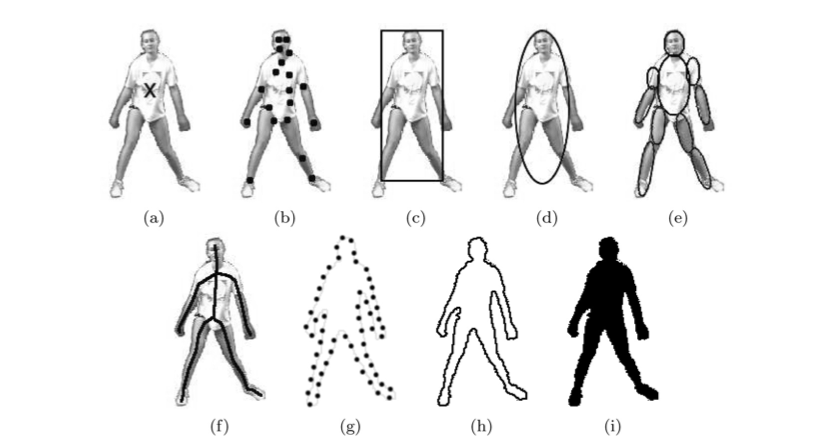
\includegraphics[scale=0.5]{figuras/2.FundamentacaoTeorica/representacao.png}
		\end{center}
		\caption{Representações de objetos rastreados. (a) Centroide, (b) múltiplos pontos, (c) representação retangular, (d) representação elíptica, (e) representação de múltiplas partes, (f) esqueleto do objeto, (g) contorno do objeto por pontos,(h) contorno completo do objeto, (i) silhueta do objeto~\cite{yilmaz}}
		\label{representacao}
	\end{figure}

	\begin{itemize}
		\item \textbf{Pontos:} o objeto é representado por um ponto, como por exemplo a centroide~\cite{veenman} da Figura \ref{representacao}(a), ou por vários pontos~\cite{serby}, como por exemplo na Figura \ref{representacao}(b). Essa representação é mais adequada para rastreamento de objetos que ocupam uma pequena região na imagem~\cite{yilmaz};

		\item \textbf{Formas geométricas primitivas:} o objeto é representado por formas geométricas simples como um retângulo ou uma elipse, como mostrados nas Figuras \ref{representacao}(c) e (d)~\cite{comaniciu}. Essa representação é mais adequada para simples objetos rígidos~\cite{yilmaz};

		\item \textbf{Silhueta e Contorno:} representação por contorno define os limites de um objeto, como mostrado nas Figuras \ref{representacao}(g) e (h). A região interna do contorno é chamada de Silhueta, como mostrado na Figura \ref{representacao}(i). Essa representação é mais adequada para rastrear objetos complexos de forma não rígida~\cite{yilmaz, yilmaz2}. Ela é popular devido a sua simplicidade. A silhueta ou contorno de um objeto pode ser obtida definindo métodos de limiarização ou subtração, podendo ser utilizada tanto com imagens 2D quanto 3D. A representação 2D geralmente é mais simples~\cite{moeslund};

		\item \textbf{Modelos de formas articuladas:} objetos articulados são compostos por partes do corpo que se ligam por meio de juntas. Para representar objetos articulados, utiliza-se figuras geométricas para cada parte do corpo, como mostrado na Figura \ref{representacao}(e)~\cite{yilmaz};

		\item \textbf{Modelos de esqueletos:} modelos de esqueletos são extraídos do objeto rastreado, como mostrado na Figura \ref{representacao}(f). Essa representação pode ser utilizada tanto para objetos articulados rígidos quanto não rígidos~\cite{yilmaz};
	\end{itemize}

	Para rastreamento de pessoas a representação por meio de contorno ou silhuetas são as mais adequadas~\cite{yilmaz}.

	O rastreamento de várias pessoas de maneira simultânea é considerada uma tarefa muito complexa. As representações das pessoas rastreadas podem se dividir ou fundir em novas representações devido a possíveis oclusões ou ruídos na imagem, e a aparência do objeto pode variar devido a sombras e mudanças da iluminação~\cite{moeslund}.

%%%%%%%%%%%%%%%%%%%%%%%%%%%%%%%%%%%%%%%%%%%%%%%%%%%%%%%%%%%%%%%%%%%%%%%%%%%%%%%%%%%%%%%%%%%%%%%%%%%%%%%%%%%%%%%

\subsection{Características para rastreamento}

	A seleção das características é uma tarefa crítica para o rastreamento e está fortemente relacionada com a representação do objeto. Em geral, a seleção procura as características mais singulares para que o objeto rastreado seja facilmente distinguido~\cite{yilmaz}. As características mais comuns utilizadas atualmente são:

	\begin{itemize}
		\item \textbf{Cor:} a cor do objeto é influenciada principalmente por duas características: a distribuição da iluminação e a propriedade de reflectância do objeto. Geralmente, a representação \textit{RGB} é utilizada para representar a cor~\cite{yilmaz};

		\item \textbf{Borda:} os limites de um objeto geram uma grande variação na intensidade na imagem e são menos sensíveis a variações na iluminação comparado com as cores. A detecção por meio das bordas é utilizada para identificar essas variações de intensidade na imagem. Os algoritmos que detectam as bordas do objeto geralmente as utilizam para representação dos mesmos~\cite{yilmaz};

		\item \textbf{Fluxo óptico:} é um campo denso de vetores de deslocamento que define a tradução de cada \textit{pixel} em uma região. Ele é calculado a partir da restrição de luminosidade, que pressupõe a constância de brilho de \textit{pixels} correspondentes nas \textit{frames} consecutivas~\cite{yilmaz, horn};

		\item \textbf{Textura:} é a medida da intensidade da variação da superfície que quantifica propriedades como suavidade e regularidade. A Textura é menos sensível a variação da iluminação comparado com a cor~\cite{yilmaz};

	\end{itemize}

De todas as características, a mais utilizada para rastreamento é a cor~\cite{yilmaz}.

%%%%%%%%%%%%%%%%%%%%%%%%%%%%%%%%%%%%%%%%%%%%%%%%%%%%%%%%%%%%%%%%%%%%%%%%%%%%%%%%%%%%%%%%%%%%%%%%%%%%%%%%%%%%%%%

\subsection{Detecção de objeto}

	Todo método de rastreamento requer um mecanismo de detecção de objetos que pode ser realizada a cada \textit{frame} obtida ou na primeira vez que o objeto aparece no vídeo. Os método mais populares são:


	\begin{itemize}
		\item \textbf{Detector de pontos:} esses detectores são usados para encontrar pontos de interesses dentro da imagem que tem uma expressiva textura na sua respectiva localização. Pontos de interesse são amplamente usados no contexto do movimento e no rastreamento. A qualidade desejável para o ponto de interesse é que seja invariante diante das mudanças de iluminação e ângulo de visão da câmera~\cite{yilmaz}.
	
		\item \textbf{Subtração de fundo:} é um método popular para segmentação de movimento, especialmente nas situações em que o plano de fundo é relativamente estático. Ele detecta as regiões de movimento na imagem obtendo a diferença \textit{pixel} a \textit{pixel} entre a \textit{frame} corrente e a \textit{frame} referente ao plano de fundo~\cite{weiming}. Geralmente, um algoritmo de componentes conectadas é aplicado para obter regiões conectadas que correspondem a um objeto~\cite{yilmaz}.

		\item \textbf{Segmentação:} o objetivo do algoritmo de segmentação é particionar a imagem em regiões com certo grau de similaridade. Todo algoritmo de segmentação tem dois problemas: o critério para definir uma boa partição e o método para arquivar particionamentos eficientes~\cite{yilmaz, shi}.

		\item \textbf{Aprendizagem supervisionada:} a detecção de objetos pode ser feita pelo aprendizado automático de diferentes objetos de um conjunto de exemplos por meio de um mecanismo de aprendizado. Esse aprendizado requer o armazenamento de um um conjunto de \textit{templates}. A partir desse conjunto de informações, o algoritmo gera uma função que mapeia as possíveis entradas para as saídas desejadas. Um problema padrão é a classificação onde a função gera um valor contínuo a partir de um determinado comportamento do objeto. No contexto da detecção de objetos as informações armazenadas são compostas por um par de características de objetos e uma classe associada onde ambos os valores são manualmente definidos. Seleção de características tem um papel importante no desempenho da classificação, portanto, é importante usar um conjunto de características que seja possível discriminar uma classe das outras~\cite{yilmaz}.
	\end{itemize}

%%%%%%%%%%%%%%%%%%%%%%%%%%%%%%%%%%%%%%%%%%%%%%%%%%%%%%%%%%%%%%%%%%%%%%%%%%%%%%%%%%%%%%%%%%%%%%%%%%%%%%%%%%%%%%%

\subsection{Rastreamento de objeto}

	O objetivo do rastreamento de objetos é conhecer a trajetória do mesmo no tempo localizando sua posição em cada \textit{frame}. O rastreamento de objetos também pode prover a região completa na imagem ocupada pelo objeto a cada instante~\cite{yilmaz}. 

	As atividades de detecção de objetos e de estabelecimento de correspondências entre os objetos e as instâncias dos \textit{frames} podem ser realizadas tanto separadamente como concomitantemente. No primeiro caso, as prováveis regiões de objetos são obtidas e o rastreador encontra correspondência entre os objetos e os \textit{frames}. No último caso, as prováveis regiões e as correspondências são feitas juntas e estimadas pela atualização iterativa da localização do objeto e de regiões de informações obtidos dos \textit{frames} anteriores~\cite{yilmaz}.

	Os métodos de rastreamento de objetos mais utilizados atualmente são:

	\begin{itemize}
		\item \textbf{Rastreamento de pontos:} os objetos detectados a cada frame são representados por pontos e a associação entre os pontos é feita com base no estados anterior do objeto que pode incluir a posição e o movimento. Essa abordagem requer um mecanismo externo para detectar o objeto a cada \textit{frame}~\cite{yilmaz};

		\item \textbf{Rastreamento de \textit{kernel}}: os objetos são rastreados pelo cálculo do movimento do \textit{kernel} em \textit{frames} consecutivas. Esse movimento geralmente esta na forma de transformações paramétricas como translação e rotação. \textit{Kernel} se refere ao formato ou aparência do objeto~\cite{yilmaz}.

		\item \textbf{Rastreamento de silhuetas:} o rastreamento é feito estimando a região do objeto a cada \textit{frame}. Esse método utiliza informação contida dentro da região do objeto. Esta informação pode ser na forma de densidade de aparência e modelos de forma que estão, geralmente, na forma de mapas de borda. Dado os modelos de objeto, silhuetas são rastreadas por qualquer forma de correspondência ou evolução de contorno. Ambos os métodos podem ser essencialmente considerados como segmentação de objetos aplicada no domínio temporal utilizando os priores gerados a partir dos \textit{frames} anteriores~\cite{yilmaz}.
	\end{itemize}

	Com os objetos rastreados, para obtermos a posição dos mesmos devemos obter informações de profunidade. Na próxima seção falaremos sobre como essas informações são obtidas utilizando imagens de profunidade.





	\section{Localização}
\label{sec:luz-estruturada}

	Calcular a distância de vários pontos na cena relativa a posição da câmera é uma
	importante tarefa de sistemas de computação visual~\cite{jain}. Para isso,
	deve-se obter informações de profundidade das entidades em interesse. Essas
	informações podem ser obtidas utilizando imagens de intensidade ou de
	profundidade.
	
	Uma maneira comum de se obter informações de profundidade de imagens de
	intensidade é adquirir um par de imagens usando duas câmeras deslocadas entre si
	por uma distância conhecida. Como alternativa, duas ou mais imagens obtidas de
	uma câmera em movimento também pode ser utilizadas para calcular informações de
	profundidade~\cite{jain}. Esse método é conhecido como \textit{Stereo Vision} e
	necessita ser bem calibrado.  Além disso, os algoritmos que o implementa
	geralmente são computacionalmente caros e não funcionam em ambiente com baixa
	condição de iluminação~\cite{fall-detection}.
	
	Informações de profundidade também podem ser obtidas indiretamente através de
	imagens de intensidade utilizando sinais na imagem, como sombreamento e
	textura~\cite{jain}.
	
	Em contraste com imagens de intensidade, imagens cujo valor em cada pixel é uma
	função da distância do ponto correspondente na cena do sensor são chamadas de
	imagens de profundidade, exemplificada na Figura \ref{depthimage}. Tais imagens
	podem ser adquiras diretamente utilizando sensores específicos~\cite{jain}.
	Alguns dos métodos mais conhecidos são:

	\begin{figure}[htb]
		\begin{center}
			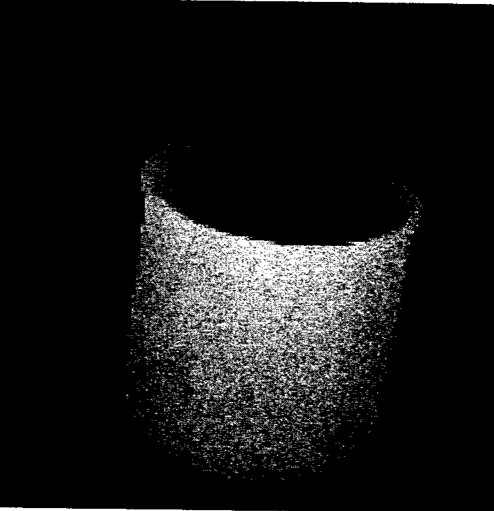
\includegraphics[scale=0.3]{figuras/2.FundamentacaoTeorica/depthimage.png}
		\end{center}
		\caption{Imagem de profundidade de uma caneca de café~\cite{jain}.}
		\label{depthimage}
	\end{figure}

	\begin{enumerate}
		\item \textbf{Triangulação:} utiliza as propriedades geométricas do triângulo
		para calcular a localização de entidades. Pode ser dividida em duas
		subcategorias: lateração e angulação. Lateração computa a posição de uma
		entidade estimando sua distância de múltiplos ponto de referência. Calcular a
		posição de uma entidade em duas dimensões requer estimativas de distância de
		três pontos não colineares como mostrado na Figura \ref{fig:lateration}. Já em
		três dimensões são necessários quatro pontos não coplanares. Ângulação utiliza
		ângulos para determinar a distância da entidade. Em geral, ângulação em duas
		dimensões requer estimativas de dois ângulos e a estimativa da distância entre
		dois pontos de referência como mostrado na Figura
		\ref{fig:angulation}~\cite{triangulacao};
		
		\begin{figure}[htb]
			\begin{center}
				\subfloat[Lateração] {
					\label{fig:lateration}
					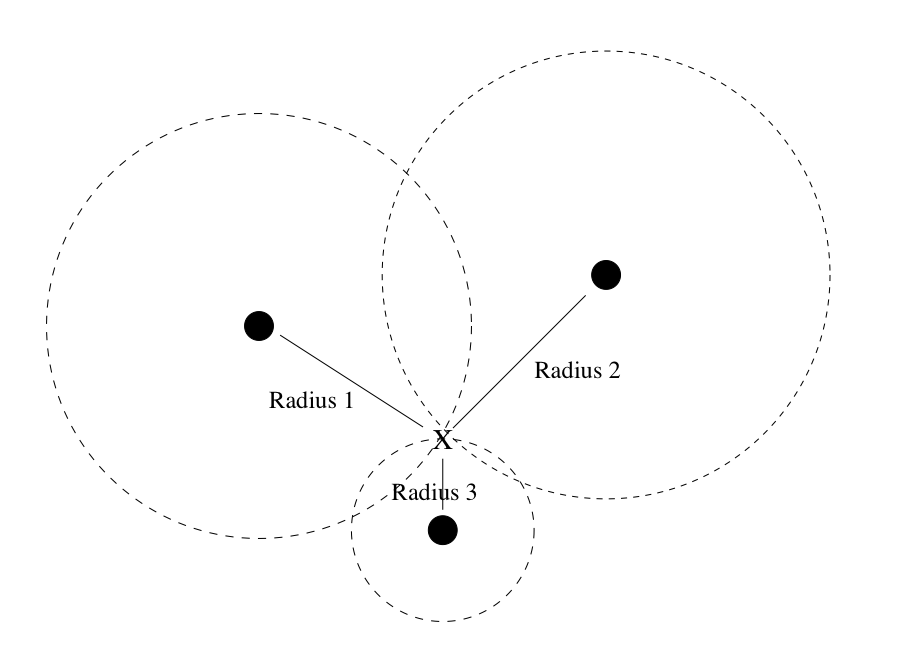
\includegraphics[width=0.45\textwidth]{figuras/2.FundamentacaoTeorica/lateration.png}}
				\subfloat[Angulação] {
					\label{fig:angulation}
					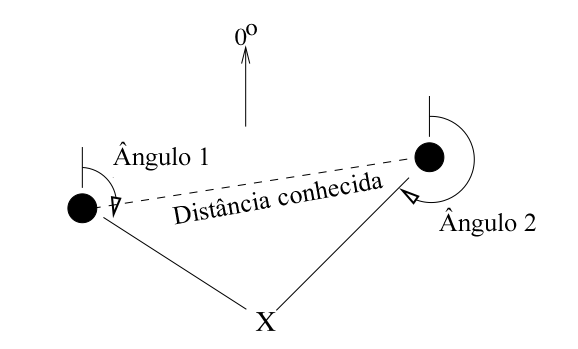
\includegraphics[width=0.45\textwidth]{figuras/2.FundamentacaoTeorica/angulation.png}}
			\end{center}
			\caption{ (a) Determina a distância em duas dimensões utilizando lateração.
			Requer a distância entre a entidade $\displaystyle X$ e três pontos de referência não colineares~\cite{triangulacao}.}
			(b) Exemplo de uma angulação em duas dimensões em que se localiza a
			entidade $\displaystyle X$ utilizando ângulos relativos a um vetor de
			referência $\displaystyle 0º$ e a distância entre dois pontos de referência~\cite{triangulacao}.}
		\end{figure}

		\item \textbf{Tempo de Vôo (TOF - \textit{Time of flight}):} a distância até a
		entidade é calculada observando a diferença de tempo entre o pulso
		eletromagnético transmitido e recebido. A informação de profundidade também pode
		ser obtida através da detecção da diferença de fase entre as ondas transmitidas
		e as recebidas de um feixe de amplitude modulada~\cite{jain, fall-detection}.
		Câmeras TOF provêem imagens de profundidade com melhor acurácia em relação ao
		método de \textit{Stero Vision}, porém são muito caras e pouco
		acessíveis~\cite{fall-detection};
		
		\item \textbf{Luz Estruturada:} uma imagem de
		profundidade não pode ser obtida utilizando somente um sensor de vídeo. Porém,
		adicionando uma textura artificial na cena, como na
		Figura~\ref{fig:structured-light}, uma imagem de profundidade pode ser
		recuperada. Esse princípio consiste na projeção de pontos de luz infra-vermelhos
		na cena que são recuperados por uma câmera infra-vermelha que lê a textura.
		Trata-se de um método mais acessível que o TOF, porém é pouco eficiente
		para estimar a distância dos pontos nas bordas dos objetos e em áreas muito
		longe do sensor~\cite{fall-detection};
		
		\begin{figure}[htb]
			\begin{center}
				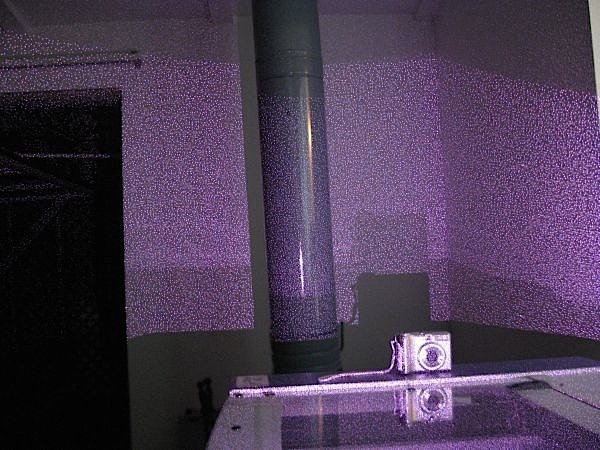
\includegraphics[width=0.45\textwidth]{figuras/2.FundamentacaoTeorica/structured-light.jpg}
			\end{center}
			\caption{Exemplo de uma textura artificial adicionada a cena por meio de
			pontos de luz infra-vermelha utilizando o método Luz Estruturada~\cite{img-strutuctured-light}.}
			\label{fig:structured-light}
		\end{figure}
	\end{enumerate}

	Imagens de profundidade são úteis devido a sua especificação explícita de
	valores de profundidade. Ao mesmo tempo acreditava-se que se a informação de
	profundidade fosse disponibilizada de maneira explícita, o processamento
	posterior da imagem seria facilitado. Tornou-se claro que a informação de
	profundidade ajuda, porém a tarefa básica de interpretação de imagens mantém
	todas as suas dificuldades~\cite{jain}.



	

\chapter{Reconhecimento Facial}

	Neste capítulo será apresentada uma abordagem conceitual sobre reconhecimento facial, uma vez que esse tópico consiste no alicerce de nosso trabalho. 

	Será apresentado também os conceitos gerais sobre biometria e sobre as características biométricas existentes.

	Sobre reconhecimento facial, será apresentado os conceitos gerais e conceitos mais específicos das diferentes etapas do processo de reconhecimento: detecção de faces e reconhecimento das mesmas. Além desses conceitos, será apresentado alguns métodos utilizados atualmente em cada uma dessas etapas.


	\section{Biometria}

As abordagens de identificação pessoal que utilizam ``alguma coisa que você sabe'', como Número de Indetificação Pessoal (PIN - ``Personal Identification Number''), ou ``alguma coisa que você tenha'', como um cartão de identificação, não são confiáveis o suficiente para satisfazer os requisitos de segurança de um sistema de transações eletrônicas porque não têm a capacidade de diferenciar um usuário legítimo de um impostor que adiquiriu de forma ilegal o privilégio de acesso \cite{hong}. Esta fragilidade pode ser evitada se utilzarmos o nosso corpo como chave do sistema. Alguns traços fisícos ou comportamentais são muito mais complicados de serem forjados que uma cadeia de caracteres \cite{drovetto}.

Biometria é uma tecnologia utilizada para identificação de um indivíduo baseado em suas características físicas ou comportamentais, baseia-se em ``alguma coisa que você é ou faz'' para realizar a identificação e, por isso, tem a capacidade de diferenciar entre um indivíduo legítimo de um impostor \cite{hong}. As características físicas estão relacionadas a composição do corpo humano e seu formato e as comportamentais estão relacionadas ao comportamento das pessoas \cite{drovetto}. A figura \ref{caracteristicasBiometricas}contém alguns exemplos desses dois tipos diferentes de características biométricas.

	\begin{figure}[hbt]
		\begin{center}
			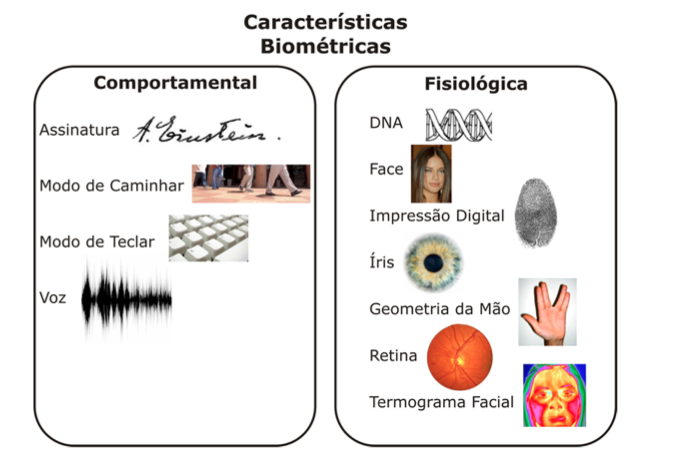
\includegraphics[height=11cm,width=17cm]{figuras/2.FundamentacaoTeorica/caracteristicasBiometricas.png}
		\end{center}
		\caption{Exemplos de algumas características biométricas \cite{drovetto}.}
		\label{caracteristicasBiometricas}
	\end{figure}

Teoricamente, qualquer característica física/comportamental pode ser utilizada para identificação caso siga alguns dos seguintes requisitos \cite{milene}: 

	\begin{enumerate}
		\item \textbf{universidade}: qualquer pessoa pode ser avaliada sobre essa característica;
		\item \textbf{singularidade}: dada duas pessoas distinas, elas não podem ter a mesma característica;
		\item \textbf{permanência}: a característica não pode mudar de acordo com o tempo;
		\item \textbf{exigibilidade}: significa que a característica pode ser mensurada quantitativamente;
	\end{enumerate}

Porém, na prática também são considerados outros requisitos \cite{milene}:

	\begin{enumerate}
		\item \textbf{desempenho}: o processo de identificação deve apresentar um resultado aceitável;
		\item \textbf{aceitação}: indica em que ponto as pessoas estão dispostas a aceitar o sistema biométrico;
		\item \textbf{evasão}: refere a facilidade de ser adulterado;
	\end{enumerate}

São várias as vatangens que os sistemas biométricos têm em relação aos sistemas convencionais. Listamos as vatagens vistas como principais \cite{drovetto}:
	
	\begin{itemize}
		\item características biométricas não podem ser perdidas ou esquecidas;
		\item características biométricas são difíceis de serem copiadas, compartilhadas e distribuídas;
		\item os sistemas biométricos necessitam que a pessoa esteja presente no local da autenticação;
	\end{itemize}

Novas técnicas de reconhecimento por meio de faces, íris, retina e voz, entre outras, têm sido abordadas para aplicações em sistemas de reconhecimento automático \cite{bolle,saocarlos}. O reconhecimento facial é apenas uma das nove características biométricas utilizadas atualmente \cite{milene}. Nas tabelas \ref{tabelaRequisitosTeoricos} e \ref{tabelaRequisitosPraticos} são mostradadas as noves características e seus respectivos comportamentos baseados nos requisitos mencionados acima.
		
	\begin{table}[htb]
		\begin{center}
			\caption{Requisitos teóricos para algoritmos de reconhecimento facial \cite{milene}.}
			\begin{tabular}{|c|c|c|c|c|}
				\hline \bf Biometria & \bf Universidade & \bf Singularidade & \bf Permanência & \bf Exigibilidade \\
				\hline \hline \bf Face & Alta & Baixa & Média & Alta \\
				\hline \bf  Digital & Média & Alta & Alta & Média \\
				\hline \bf Geometria da Mão & Média & Média & Média & Alta \\
				\hline \bf ``Hand Vein'' & Média & Média & Média & Média \\
				\hline \bf Iris & Alta & Alta & Alta & Média \\
				\hline \bf ``Retina Scan'' & Alta & Alta & Média & Baixa \\
				\hline \bf Assinatura & Baixa & Baixa & Baixa & Alta\\
				\hline \bf Voz & Média & Baixa & Baixa & Média \\
				\hline \bf Termograma & Alta & Alta & Baixa & Alta \\
				\hline
			\end{tabular}
		\end{center}
		\label{tabelaRequisitosTeoricos}
	\end{table}

	\begin{table}[htb]
		\begin{center}
			\caption{Requisitos práticos para algoritmos de reconhecimento facial \cite{milene}.}
			\begin{tabular}{|c|c|c|c|}
				\hline \bf Biometria & \bf Desempenho & \bf Aceitação & \bf Evasão \\
				\hline \hline \bf Face & Baixa & Alta & Baixa\\
				\hline \bf Digital & Alta & Média &  Alta\\
				\hline \bf Geometria da Mão & Média & Média & Média\\
				\hline \bf ``Hand Vein'' & Média & Média & Alta\\
				\hline \bf Iris  & Média & Média & Alta\\
				\hline \bf ``Retina Scan'' & Alta & Baixa & Alta\\
				\hline \bf Assinatura & Baixa & Alta & Baixa \\
				\hline \bf Voz & Baixa & Alta & Baixa \\
				\hline \bf Termograma & Média & Alta & Alta \\
				\hline
			\end{tabular}
		\end{center}
		\label{tabelaRequisitosPraticos}
	\end{table}

Um sistema biométrico responde a dois eventos: um usuário é ou não quem afirma ser. Como resposta a esses eventos, o sistema pode classificar o usuário como um cliente ou um impostor. Nessa tomada de decisão pode ocorrer dois tipos de erros: uma falsa aceitação, ao aceitar um impostor, (\textit{False Acceptance} - FA) ou uma falsa rejeição (\textit{False Rejection} - FR), ao rejeitar um cliente. Baseado nesses erros, duas taxas são utilizadas para avaliar sistemas biométricos: taxa de falsa aceitação (\textit{False Acceptance Rate} - FAR) e taxa de falsa rejeição (\textit{False Rejection Rate} - FRR) \cite{drovetto}.

A FAR é a probabilidade de um sistema biométrico aceitar um impostor como cliente. Ela é calculada pela equação (2.1) em que $\displaystyle Nfa$ é o número de falsas aceitações e $\displaystyle Ni$ é o número de impostores que tentaram acessar o sistema. A variação da taxa é representada pelo intervalo fechado $\displaystyle [0,1]$, onde o valor $\displaystyle 1$ significa que todos os impostores foram falsamente aceitos e o valor $\displaystyle 0$ significa que todos impostores foram identificados como tao. Logo quando menor o FAR mais seguro o sistema é \cite{drovetto}.

	\begin{equation}
		FAR = \frac{Nfa}{Ni} \cite{drovetto}
	\end{equation} 

A FRR é a probabilidade de um sistema biométrico rejeitar um cliente e classifica-lo como impostor. Ela é calculada pela equação (2.2) em que $\displaystyle Nfr$ é o número de falsas rejeições e $\displaystyle Nc$ é o número de clientes que tentaram acessar o sistema. A variação da taxa é representada pelo intervalo fechado $\displaystyle [0,1]$, onde o valor $\displaystyle 1$ significa que todos os clientes foram falsamente rejeitados e o valor $\displaystyle 0$ significa que todo os cliente foram aceitos corretamente. Em sistemas cuja performance tem maior grau de prioridade que a segurança, deve-se reduzir a FRR para minimizar a ocorrência de falsas rejeições \cite{drovetto}.

	\begin{equation}
		FRR = \frac{Nfr}{Nc} \cite{drovetto}
	\end{equation} 

A partir dessas taxas de erro, pode-se obter outras medidas como a \textit{Equal Error Rate} (ERR). Esta corresponde a taxa de erro na qual a tanto a FAR quanto a FRR possuem o mesmo valor. Como diferentes sistemas têm comportamentos diferentes, a ERR normalmente é utilizada para uma comparação mais rigorosa entre o sistemas. Quanto menor for a ERR, mas presciso é considerado o sistema \cite{drovetto}.

	\section{Reconhecimento Facial}

O reconhecimento facial é uma das atividades mais comuns realizadas diariamente por seres vivos dotados de certa inteligência. Essa simples atividade vem despertando o interesse de pesquisadores que trabalham com Visão Computacional e Inteligência Artificial. O objetivo desses pesquisadores é de construir sistemas artificiais capazes de realizar o reconhecimento de faces humanas e a partir desta capacidade construir os mais diferentes tipos de aplicações: sistemas de vigilância, controles de acesso, definções automáticas de perfis, entre outros \cite{oliveira}.

No anos 70, os estudos do reconhecimento facial eram baseados sobre atributos faciais mensuráveis como olhos, nariz, sobrancelhas, bocas, entre outros. Porém, os recursos computacionais eram escassos e os algoritmos de extração de características eram ineficiêntes. Nos anos 90, as pesquisas na área ressurgiram, inovando os métodos existentes \cite{hong, saocarlos} e disseminando a técnica.

Um dos motivos que incentivou os diversos estudos sobre reconhecimento facial são as vantagens que o mesmo possui em relação a impressão digital e a íris.  No reconhecimento por impressão digital, a desvantagem consiste no fato que nem todas as pessoas possuem uma impressão digital com ``qualidade'' suficiente para ser reconhecida por um sistema. Já o reconhecimento por íris apresenta uma alta confiabilidade e larga variação, sendo estável pela vida toda. Porém, a desvantagem está relacionada ao modo de captura da íris que necessita de um alinhamento entre a câmera e os olhos da pessoa \cite{saocarlos}. 

Basicamente existem duas particularidades que fazem da face uma característica biométrica bastante atrativa \cite{drovetto}:

	\begin{enumerate}
		\item A aquisição da face é feita de forma fácil e não-intrusiva;
		\item Possui uma baixa privacidade de informação: como a face é exposta constantemente, caso uma base de faces seja roubada, essas informações não representam algum risco e não possibilitam um uso impróprio;
	\end{enumerate}

Umas das maiores dificuldades dos sistemas de reconhecimento é tratar a complexidade dos padrões visuais. Mesmo sabendo que todas as faces possuem padrões reconhecidos, como boca, olhos e nariz, elas também possuem variações únicas que devem ser utilizadas para determinar as características relevantes. Outra dificuldade encontrada em relação a essas características é que elas possuem uma larga variação estatística para serem consideradas únicas para cada indivíduo. O ideal seria que a variância inter-classe seja grande e a intra-classe pequena, pois assim imagens de diferentes faces geram os códigos mais diferentes possíveis, enquanto imagens de uma mesma face geram os códigos mais similares possíveis. Portanto, estabelecer uma representação que capture as características ideias é um difícil problema \cite{saocarlos}.

Do ponto de vista geral, o recohecimento facial continua sendo um problema aberto por causa de várias dificuldades que aumentam a variância intra-classe \cite{hong}. Entre estas, destacamos as mais comuns \cite{saocarlos}:

	\begin{itemize}
		\item iluminação;
		\item ângulos e poses;
		\item expressões;
		\item comésticos e acessórios;
		\item extração da face do contexto ou do fundo;
	\end{itemize}

No contexto de identificação, o reconhecimento facial se resume no reconhecimento de um ``retrato'' frontal, estático e controlado. Estático pois os ``retratos'' utilizados nada mais são que imagens, podendo ser tanto de intensidade quanto de profunidade e controlado pois a iluminação, o fundo, a resolução dos dispositivos de aquisição e a distância entre eles e as faces são essencialmente fixas durante o processo de aquisição da imagem \cite{hong}.

Basicamente, o processo de reconhecimento facial pode ser divido em duas tarefas principais \cite{hong}:

	\begin{enumerate}
		\item Detecção de faces em imagens;
		\item Reconhecimento das faces encontradas;
	\end{enumerate}

Falaremos dessas duas tarefas separadamente nas próximas subseções.



\subsection{Detecção de Faces em imagens}
	
A primeira etapa para o reconhecimento de faces é a detecção de um rosto, e a partir daí a comparação do mesmo com modelos conhecidos pelo sistema \cite{hong, oliveira}. Em um sistema de reconhecimento facial, tanto o tempo de resposta quanto a confiabilidade desta etapa influência diretamente no desempenho e o emprego deste sistema \cite{oliveira}.

A detecção de faces é definida como o processo que determina a existência ou não de faces em uma imagem e uma vez encotrada alguma face, sua localização deve ser apontada através de um enquadramento ou através de suas coordenadas dentro da imagem \cite{oliveira}. A figura \ref{enquadramentoRosto} representa um exemplo da detecção de uma face em uma imagem.

	\begin{figure}[hbt]
		\begin{center}
			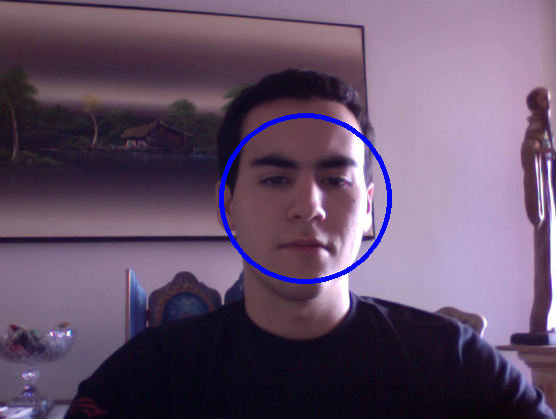
\includegraphics[height=9.5cm,width=12.5cm]{figuras/2.FundamentacaoTeorica/enquadramentoRosto.png}
		\end{center}
		\caption{Exemplo de um processo de detecção de uma face em uma imagem.}
		\label{enquadramentoRosto}
	\end{figure}

O processo de detecção de faces geralmente é pelas seguintes razões mostradas a seguir:

	\begin{enumerate}
		\item \textbf{Pose}: as imagens de uma face podem variar de acordo com a posição relativa entre a camêra e a face (frontal, 45 graus, perfil, ``de cabeça para baixo''), e com isso algumas características da face, como olhos e nariz, podem ficar parcialmente ou totalmente ocultadas \cite{yang}.
		\item \textbf{Presença de acessórios}: características faciais básicas importantes para o processo de detecção podem ficar ocultadas pela presença de acessórios, como óculos, bigode, barba, entre outros \cite{oliveira, yang}. 
		\item \textbf{Expressões faciais}: embora a maioria das faces apresente estruturas semelhantes (olhos, bocas, nariz, entre outros) e são dispostas aproximadamente na mesma configuração de espaço, pode haver um grande número de componentes não rigídos e texturas diferentes entre as faces. Um exemplo são as flexibilizações causadas pelas expressões faciais \cite{oliveira, yang};
		\item \textbf{Obstrução}: faces podem ser obstruídas por outros objetos. Em uma imagem com várias faces, uma face pode obstruir outra \cite{yang}.
		\item \textbf{Condiçoes da imagem}: a não previsibilidade das condições da imagem em ambientes sem restrições de ilimuniação, cores e objetos de fundo \cite{oliveira, yang}.
	\end{enumerate}

Atualmente, já existem diferentes métodos/técnicas de detecção de faces. Faleremos um pouco sobre os métodos baseados em imagens de itensidade e de cor e depois falaremos sobre os baseados em imagens 3D.

Um problema relacionado e muito importante é como avaliar a performance dos métodos de detecção de faces propostos. Com isso, muitas métricas foram adotadas como tempo de aprendizagem, número de amostras necessárias no treinamento e a proporção entre taxas de detecção e ``falso alarme''. Esta última é dificultada pelas diferentes definições para as taxas de detecção e falso alarme adotadas pelos pesquisadores \cite{yang}.

% ##################################################################################################################
% ##################################################################################################################
% ##################################################################################################################

\subsection{Reconhecimento das Faces encontradas}

Na etapa de reconhecimento, as faces detectadas e processadas, serão comparadas com um banco de dados de faces conhecidas. Essa comparação tem uma acurácia media de 30-90\% entre as diversas técnicas []. Esse é um forte campo de pesquisa desde a década de 90 e as técnicas se invovam ano ápos ano.

	Técnicas 2D:
	\begin{enumerate}
		\item \textbf{Eigenfaces} []
		\item \textbf{Redes Neurais} []
		\item \textbf{Fisher Faces} []
	\end{enumerate}

Com o surgimento da tecnologia 3D o reconhecimento facial se trasformou mais confiável pois a imagem 3D evita problemas comum em reconhecimentos faciais 2D como a mudança na iluminação, diferentes expressões faciais, maquiagem e orientação da cabeça.
	Técnicas 3D:
	\begin{enumerate}
		\item \textbf{``Face Recognition Homepage''} []
		\item \textbf{``3D Face Recognition''} []
		\item \textbf{``Active Appearance Models''} []
	\end{enumerate}


O Eigenface é um algoritmo de reconhecimento facial 2D simples e fácil de implementar. Os passos utilizados pelo Eigenface também são utilizados em muitos métodos avançados. Os princípios básicos por trás dele como PCA(``Principal Component Analisys'') e ``distance-based matching'' aparecem mais e mais na computação visual e aplicações diversas de maquinas inteligentes.
O Eigenface trabalha de forma simples, dada uma imagem de um rosto desconhecido e imagens do rosto das pessoas conhecidas executa as seguintes ações.
	\begin{enumerate}
		\item Computa a distância entre a nova imagem e cada uma das imagens já conhecidas.
		\item Seleciona a imagem mais proxima do novo rosto.
		\item Se a distância da nova imagem para a imagem exemplo for maior que o limite predefinido, ``reconhece'' a imagem caso contrario classifica como ``desconhecida''.
	\end{enumerate}


A distância entre as imagens é medida ponto a ponto. Esta é também chamado de distância euclidiana. Em duas dimensões (2D), a distância euclidiana entre os pontos $P_1$ e $P_2$ é dada pela fórmula $\displaystyle d_{12} = \sqrt(d_{x2} + d_{y2})$, onde $\displaystyle d_x = x_2 - x_1$ e $\displaystyle d_y = y_2-y_1$ e representada na Figura \ref{distanciaEntrePontos}.

    \begin{figure}[hbt]
		\begin{center}
			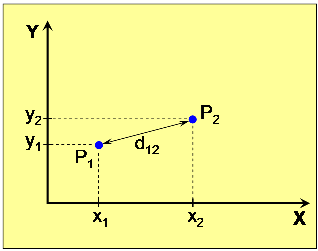
\includegraphics[height=9.5cm,width=12.5cm]{figuras/2.FundamentacaoTeorica/graficoDistanciaEntrePontos.png}
		\end{center}
		\caption{Distância Euclidiana entre dois pontos em duas dimensões.}
		\label{distanciaEntrePontos}
	\end{figure}


Imagens possuem ``ruídos'' e vamos definir ruído como qualquer coisa que atrapalhe na identificação, como por exemplo as diferenças na luminosidade. Cada pixel possui uma intensidade de ruído diferente e com cada pixel dando a sua contribuição fica muito difícil encontrar a imagem correta. Uma solução é diminuir a dimensionalidade da imagem tornando assim o ruido menor e sendo possível extrair as informações importante da imagem.

Um dos métodos existentes para redução de imagem é o ``PCA - Principal Components Analysis''.

Para se ter uma idéia do que é o PCA, vejamos um caso especial chamado de ``least squares line fit''. O lado esquerdo da Figura \ref{exemploPCA} mostra um exemplo de uma linha média entre três pontos, que são, no mapa em 2D, Los Angeles, Chicago e Nova York. Estes três pontos do mapa são quase, mas não completamente, uma única linha. Se você estava planejando uma viagem, essa relação já seria uma informação útil. Nesse sentido, uma única linha expressa algo essencial sobre seu relacionamento. A linha tem apenas uma dimensão, por isso, se podemos substituir localizações dos pontos de 2D com localizações ao longo de uma única linha, vamos ter reduzido a sua dimensionalidade.

Como eles já estão quase alinhados, uma linha pode ser traçada através deles com pouco erro. O erro no ajuste da linha é medido pela soma do quadrado da distância de cada ponto da linha. A linha de melhor ajuste é aquela que possui o menor erro.

	\begin{figure}[hbt]
		\begin{center}
			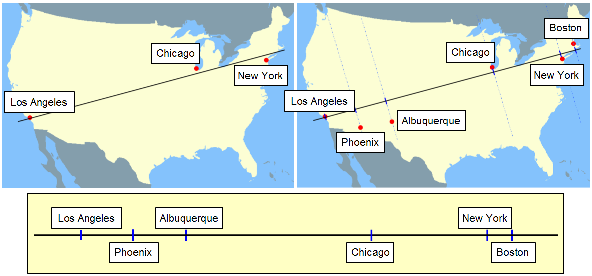
\includegraphics[height=9.5cm,width=12.5cm]{figuras/2.FundamentacaoTeorica/PCAexemploMapa.png}
		\end{center}
		\caption{Mapa exemplo para redução de dimensionalidade}
		\label{exemploPCA}
	\end{figure}

Embora a linha encontrada acima é um objeto 1D, é localizado dentro de um espaço maior, 2D, e tem uma orientação, sua inclinação. A inclinação da linha expressa algo importante sobre os três pontos. Ele indica a direção em que eles estão mais espalhados.


Se posicionarmos a origem do nosso plano cartesiano em algum lugar dessa linha, podemos escrever a equação da linha como uma simples $y = mx$, onde m é a inclinação da linha: $dy / dx$.

Quando ele é descrito desta maneira, a linha é um subespaço do espaço 2D definido pelo sistema de coordenadas. Esta descrição enfatiza o aspecto dos dados que estamos interessados, ou seja, a direção que mantém esses pontos mais separados um do outro.

Esta direção da separação máxima é chamada de primeira componente principal de um conjunto de dados. A próxima direção com máxima separação é a perpendicular a esta. Essa é a segunda componente principal. Em um conjunto de dados 2D, podemos ter no máximo duas componentes principais.

No entanto, o número de componentes principais que podemos encontrar também é limitada pelo número de pontos de dados. Para ver o porque disto, podemos pensar em um conjunto de dados que consiste de apenas um ponto. Não há sentido da separação máxima para esse conjunto de dados, porque não há nada para separar. Agora, considere um conjunto de dados com apenas dois pontos. A linha que conecta esses dois pontos é a primeira componente principal. Mas não há uma segunda componente principal, porque não há nada mais para separar, pois os dois pontos estão totalmente na linha.

Em Eigenface, cada imagem da face, de tamanho 50x50, é tratada como um ponto (com espaço dimensional de 2500). Portanto, o número de componentes principais, podemos encontrar nunca será mais do que o número de imagens de faces menos um.

Embora seja importante ter um entendimento conceitual do que as componentes principais são, você não precisa saber os detalhes de como encontrá-las para implementar o Eigenface. Essa parte já foi implementada em bibliotecas de processamento de imagens \textit{open source}, como por exemplo a bliblioteca ``OpenCV''.

Voltando ao mapa da Figura \ref{exemploPCA}, agora que nós encontramos um subespaço 1D, temos uma maneira de converter os pontos em 2D para 1D. Esse processo se chama projeção. Para projetar um ponto do mapa para a linha, você encontra o ponto da linha que está mais próximo do ponto 2D. Essa é sua projeção.

Há uma função no ``OpenCV'' para projetar os pontos sobre um subespaço, então, novamente, você só precisa de um entendimento conceitual. Você pode deixar os detalhes algorítmicos para a biblioteca.

As marcas azuis na Figura \ref{exemploPCA} mostram as localizações no subespaço das três cidades que definiram a linha. Outros pontos 2D também pode ser projetado para esta linha. O lado direito da Figura \ref{exemploPCA} mostra a localização prevista para Phoenix, Albuquerque, Boston.

Em Eigenface, a distância entre duas imagens é a distância euclidiana entre os pontos projetados em um subespaço, ao invés da distância no espaço original da imagem de 2500 dimenções. A distância entre as faces neste subespaço de menor dimensão é a técnica utilizada para melhorar a relação sinal / ruído.

Muitas técnicas avançadas de reconhecimento de face são extensões deste conceito básico. A principal diferença entre Eigenface e estas técnicas avançadas é o processo de definição do subespaço. Em vez de usar PCA, o subespaço pode ser baseada em Análise de Componentes Independentes (ICA) ou em Análise Discriminante Linear (LDA), e assim por diante.

Em nossa definição de uma linha como um subespaço 1D, usamos X e Y coordenadas para definir m, que é sua inclinação em 2D. Quando m é um componente principal de um conjunto de pontos, ela é chamada de autovetor ou ``eingenvector'', daí o nome eigenface. 

Para o reconhecimento facial em imagens de 50x50, cada autovetor representa a inclinação de uma linha em um espaço de 2.500 dimenções. Como no caso 2D, precisamos de todas as 2.500 dimensões para definir a inclinação de cada linha. Embora seja impossível visualizar uma linha em muitas dimensões, podemos visualizar os autovetores de uma maneira diferente. Podemos converter as suas 2.500 dimenções em uma simples imagem usando a sua ``inclinação'' para colocar cada pixel valor em seu local correspondente. Quando fazemos isso, obtemos imagens ``facelike'' chamadas de eigenfaces.

Eigenfaces é um método interessante para dar-nos alguma intuição sobre os componentes principais para o nosso conjunto de dados. O lado esquerdo da Figura \ref{exemploEigenfaces} mostra as imagens das faces de dez pessoas. Estas imagens foram encontradas no ``Yale Face Database B (referências 4 e 5)''. Ele contém imagens de rostos com uma variedade de condições de iluminação. Foram usadas sete imagens de cada uma dessas dez pessoas para criar um subespaço PCA. 

O lado direito da Figura \ref{exemploEigenfaces} mostra os seis primeiros componentes principais deste conjunto de dados, apresentados como eigenfaces. O eigenfaces muitas vezes têm um olhar fantasmagórico, porque combinam elementos de várias faces. As regiões de pixels mais brilhantes e as regiões mais escuras em cada imagem foram os que mais contribuíram para esse componente principal. 

	\begin{figure}[hbt]
		\begin{center}
			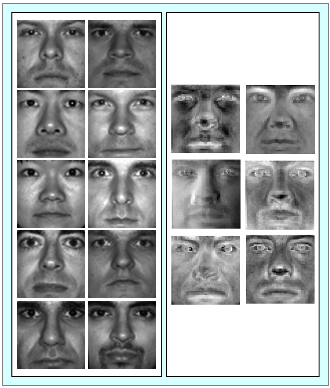
\includegraphics[width=12cm]{figuras/2.FundamentacaoTeorica/eigenfaces.png}
		\end{center}
		\caption{Direita: imagens de rosto para dez pessoas. Esquerda: os seis primeiros componentes principais, visto como eigenfaces.}
		\label{exemploEigenfaces}
	\end{figure}

Os principais componentes que encontra APC são os rumos da maior variação nos dados. Um dos pressupostos na Eigenface é que a variabilidade nas imagens subjacente corresponde à diferença entre as faces individuais. Esta suposição é, infelizmente, nem sempre válido. A Figura \ref{exemplosImagensIluminacaoo} mostra os rostos de duas pessoas. A face de cada indivíduo é apresentada em quatro diferentes condições de iluminação.

Estas imagens são também do ``Yale Face Database B''. Na verdade, eles são imagens de faces de duas das dez pessoas mostrado na Figura \ref{exemploEigenfaces}. Você pode dizer qual é qual? Eigenface não pode. Quando a iluminação é muito variável, Eigenface muitas vezes não o faz melhor palpite aleatório faria.

	\begin{figure}[hbt]
		\begin{center}
			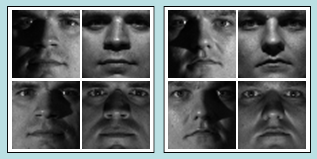
\includegraphics[width=14cm]{figuras/2.FundamentacaoTeorica/exemplosImagensIluminacaoo.png}
		\end{center}
		\caption{Face imagens de dois indivíduos. A face de cada indivíduo é apresentada em quatro diferentes condições de iluminação. A variabilidade devido à iluminação aqui é maior do que a variabilidade entre os indivíduos. Eigenface tende a confundir as pessoas quando os efeitos de iluminação são fortes.}
		\label{exemplosImagensIluminacaoo}
	\end{figure}


%Como mencionado em cima, essa idéia básica - redução de dimensionalidade seguido pelo cálculo da distância em um subespaço - é amplamente utilizado no trabalho de visão computacional. Também é utilizado em outros ramos da AI. Na verdade, é uma das principais ferramentas para gerenciar a complexidade e para encontrar padrões escondidos dentro de enormes quantidades de dados do mundo real.




% Os métodos baseados em imagens de intensidade e cor podem ser divididos em 4 categorias \cite{yang}:

% 	\begin{enumerate}
% 		\item \textbf{``Knowladge-based methods'':} métodos, desenvolvidos principalmente para localização facial, beaseados em regras derivadas do conhecimento dos pesquisadores do que constitui uma típica face humana. Normalmente, captura as relações existentes entre as características faciais. É fácil econtrar regras que descrevem as caracterísicas faciais. Por exemplo, uma face sempre é constituída por dois olhos simétricos, um nariz e uma boca. As relações entre essas características podem ser representadas pelas distâncias relativas e posições.  \cite{yang};

% 		\item \textbf{``Feature invariant approaches'':} esses algoritmos tem como objetivo principal encontrar as características estruturais que existem mesmo quando a postura, ``ponto de vista'', condições de iluminação variam. E por meio dessas características localizar a face. São desenvolvidos principalmente para localização facial \cite{yang};

% 		\item \textbf{``Template matching methods'':} vários padrões comuns de um rosto são armazenados tanto para descrever o rosto como um todo quanto para descrever as características faciais separadamente. As correlações entre as imagens de entrada e os padrões armazenados são comuptados para detecção. Esses métodos são desenvolvidos para serem utlizados como localização e detecção facial \cite{yang};

% 		\item \textbf{``Appearence-based methods'':} Em contraste com os métodos do item anterior, os modelos são retirados de um conjunto de imagens de treinamento que devem capturar a variabilidade da face. Esses modelos retirados são utilizados para detecção. São métodos desenvolvidos principalmente para detecção de faces \cite{yang};

% 	\end{enumerate}






























\chapter{Trabalhos Correlatos}

Neste capítulo serão analisados alguns projetos que focam no rastreamento, identificação e localização de pessoas em um ambiente inteligente. 

Alguns dos projetos estudados utilizam técnicas de identificação e rastreamento multimodais. Estas são compostas por informações redundantes providas por alguns tipos diferentes de sensores como, por exemplo, sensores de áudio e vídeo que fornecem dados audiovisual  das pessoas no ambiente.

Mesmo assim, somente as técnicas de identificação, localização e rastreamento monomodais que utilizarem imagens (cor, intensidade ou profundidade) como entrada serão descritas e analisadas.

Dentre os projetos estudados, destacam-se os seguintes projetos....(falar o pq).

\section{Projeto CHIL}

O Projeto CHIL (\textit{Computers in the Human Interaction Loop})~\cite{chil, computerschil} envolve uma rede de quinze laboratórios internacionais de pesquisa acadêmica e industrial. Eles colaboram entre si conduzindo pesquisas que tem por objetivo ajudar a pessoas de forma proativa durante suas atividades diárias no ambiente de trabalho. Em especial, o projeto foca no desenvolvimento de sistemas que auxiliam as interações entre grupos de pessoas como, por exemplo, sistemas que facilitam a colaboração em reuniões e em salas de palestras. Dentre os protótipos que foram desenvolvidos no projeto destacam-se um ambiente de trabalho perceptivo e colaborativo e um sistema perceptivo de assistência a um escritório virtual.

Este projeto utiliza uma combinação de algoritmos monomodais para criar um sistema de rastreamento e identificação multimodal utilizando dados audiovisuais das pessoas no ambiente. Contudo, apesar do foco desta monografia ser identificação, rastreamento e localização utilizando imagens, vale salientar que o Projeto CHIL representa uma das primeiras tentativas de realizar e avaliar sistematicamente rastreamento acústico com uma rede distribuída de microfones. Portanto, os relatos a seguir serão relativos somente às investigações que utilizam dados visuais (imagens) para rastreamento e identificação. Referente a localização das pessoas no ambiente, o projeto focou somente na localização das pessoas que ``falam''~\cite{speaker-localization}.

\subsection{Rastreamento de pessoas}

As pesquisas sobre rastreamento de pessoas no âmbito do Projeto CHIL concentraram-se principalmente no rastreamento de pessoas dentro de um ambiente inteligente. Neste contexto, o rastreamento tem o objetivo de determinar,  de maneira contínua, as coordenadas dos ocupantes na imagem capturada.

Os sensores utilizados no ambiente inteligente do Projeto CHIL incluem:	
	\begin{itemize}
		\item um mínimo de quatro câmeras fixas instaladas nos cantos do ambiente, com campos de visão sobrepostos;
		\item uma câmera com grande ângulo de visão fixa com vista para o ambiente inteiro;
		\item três arrays de microfones em forma de T de 4 canais cada;
		\item um microfone de Mark III de 64 canais.
	\end{itemize}

Era esperado que essa grande quantidade de sensores disponíveis pudesse ser vista como uma vantagem, por oferecerem alta redundância nas informações capturadas e boa cobertura do ambiente minimizando assim problemas como oclusão. Porém, foi relatado que tal redundância se tornou um grande desafio, pois surgiram problemas relativo à sincronização dos dados, transferência de processamento distribuído, fusão de espaço-temporal, entre outros.

Inicialmente, os sistemas do Projeto CHIL eram de uma única modalidade com inicialização manual, utilizando recursos simples e rastreamento de no máximo uma pessoa. Estes sistemas evoluíram para um sistema totalmente automático, com auto-inicialização, em tempo real, utilizando uma combinação de recursos capaz de rastrear alvos múltiplos.

Sobre os algoritmos de rastreamento visual, duas abordagens principais foram seguidas pelos vários sistemas de rastreamento desenvolvidos no Projeto CHIL:

	\begin{enumerate}
		\item Abordagem baseada em modelos, em que um modelo 3D do objeto rastreado é mantido renderizando-o nos pontos de vista da câmera.~\cite{chilref1,chilref2,chilref3}.
		\item Abordagem orientada a dados, onde sistemas de rastreamento 2D operam de forma independente sobre os diferentes ângulos de visão das câmeras e os dados do rastreamento pertencentes a um mesmo alvo são coletados no formato de um rastreamento 3D~\cite{chilref4,chilref5}.
	\end{enumerate}	

 Em termos de desempenho, foi observado que a abordagem baseada em modelos (1) geralmente prevê uma melhor acurácia, porém menos precisão do que a abordagem orientada a dados (2). Por outro lado, o tratamento das oclusões e da associação dos dados dos sistemas de rastreamentos independentes são as desvantagens do modelo orientado a dados. Foi identificado,  nesse projeto, que rastrear rostos ao invés de corpos inteiros diminui o impacto desses problemas.

 Foi observado que a abordagem baseada em modelos também facilita a incorporação de diversos tipos de recursos, como segmentos de primeiro plano, histogramas de cor, etc., que aumentam a robustez do rastreamento. Contudo, as dificuldades encontradas nesta abordagem se resumem na inicialização automática e na atualização dos modelos das pessoas.

 Os testes do sistema de rastreamento desenvolvido no Projeto CHIL foram feitos utilizando os dados dos seminários e reuniões do próprio projeto.

% As abordagens de rastreamento por meio de áudio e vídeo foram combinas em um rastreamento multimodal. Esse rastreamento multimodal é, notavelmente, baseado em filtro de partículas uma vez que permitem uma integração flexível de recursos através dos sensores~\cite{chil}.

% No rastreamento multimodal, era esperado que a fusão dos diferentes tipos de dados proveria resultados mais precisos, eliminando, assim, os efeitos de decisões erradas tomadas por algum rastreamento monomodal. Porém, não aconteceu o que se esperava. O rastreamento multimodal é altamente dependente das tarefas e dados em mãos, e exige um cuidadoso equilíbrio na disponibilidade e qualidade dos dados~\cite{chil}.

\subsection{Identificação de pessoas}


A fim de realizar a identificação de pessoas de forma natural e implícita em um ambiente inteligente, sensores distribuídos no ambiente devem monitorar continuamente o espaço de modo que o sistema de identificação opere em segundo plano sem necessitar de atenção e cooperação dos usuários. 

A equipe do Projeto CHIL desenvolveu sistemas de reconhecimento facial tendo em vista que a face é uma característica biométrica que permite uma identificação de forma natural e implícita, conforme mencionado na Seção~\ref{sec:biometria}. 

Na tentativa de realizar o reconhecimento facial das pessoas presentes no ambiente inteligente, vários desafios foram encontrados no Projeto CHIL, como: grande variação da iluminação, sensores com baixa resolução, oclusão visual. Além disso dependendo da localização e distância dos sensores da pessoa a ser identificada os dados recebidos podem variar. Foi observado, também, que o fato das pessoas possuírem diferentes expressões faciais, cortes de cabelo, maquiagem, entre outros, dificultava ainda mais a tarefa. Entretando, apesar de todos esses desafios, foi notado que o reconhecimento facial podia ser realizado de forma robusta utilizando múltiplos sensores no ambiente.

O sistema de identificação do Projeto CHIL utiliza sequências de imagens fornecidas pelas várias câmeras no ambiente inteligente. A cada $\displaysyle 200ms$ imagens das caixas delimitadoras das faces (uma maneira de apontar a localização da face na imagem por meio de um enquadramento) e posições dos centros dos olhos são extraídas. O canto inferior direito da Figura~\ref{chil} exemplifica a imagem da face extraída de uma pessoa no ambiente.

As faces extraídas são, então, alinhadas utilizando os centros dos olhos ou as caixas delimitadoras das faces. Para obter robustez e minimizar erros, o sistema gera algumas imagens adicionais alinhadas modificando rótulos do centro dos olhos ou os rótulos das caixas delimitadoras das faces.

	\begin{figure}[hbt]
		\begin{center}
			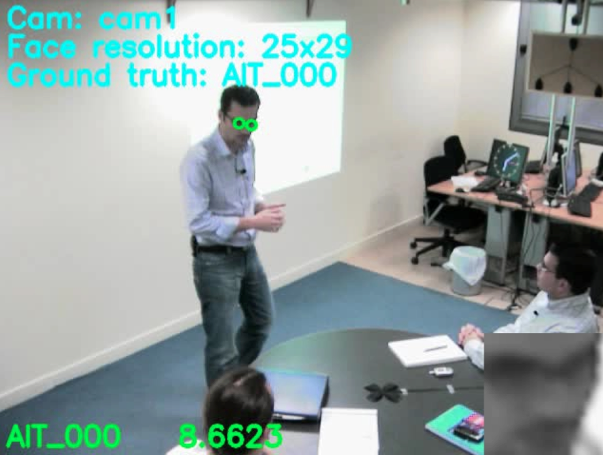
\includegraphics[scale=0.4]{figuras/3.TrabalhosCorrelatos/chil.png}
		\end{center}
		\caption{Exemplo do sistema de identificação facial do Projeto CHIL~\cite{chil}.}
		\label{chil}
	\end{figure}


No Projeto CHIL testou-se diferentes abordagens para reconhecimento facial. Uma delas realiza reconhecimento baseado em aparência utilizando transformada discreta de cosseno (DCT - \textit{Discrete Cosine Transform})~\cite{chilref6, chilref7}. Abordagens baseadas em PCA (\textit{Principal Component Analisys}) também foram testadas, utilizando como medida da distância entre imagens uma versão modificada da distância euclidiana utilizando pesos~\cite{chilref8, chilref9}.  Foi testado também uma abordagem baseada em análise discriminante linear (LDA - \textit{Linear Discrimant Analysis}), mas sem sucesso pois as imagens das faces obtidas não eram linearmente separáveis~\cite{chilref8, chilref9}. 

Todas as abordagens testadas utilizam um classificador do ``vizinho'' mais próximo. As decisões obtidas dos vários pontos de vista das várias câmeras utilizando tal classificador são, então, combinados por meio de uma regra de soma ponderada~\cite{chilref8, chilref9}.

Experimentos realizados no projeto, utilizando os mesmos métodos para extração da face e normalização, mostraram que a abordagem baseada em aparência utilizando DCT apresentou os melhores resultados. Além disso, foi observado que selecionando somente as imagens frontais de faces, ao invés de todas as amostras disponíveis, como imagens de perfil, reduz a performance do sistema de reconhecimento. 

%%%%%%%%%%%%%%%%%%%%%%%%%%%%%%%%%%%%%%%%%%%%%%%%%%%%%%%%%%%%%%%%%%%%%%%%%%%%%%%%%%%%%%%%%%%%%%%%%%%%%%%%%%%%%%%%%%%%%%%%%%%%%%%%%%%%%%%%%%%%%%%%%%%%%%%%%%%%%%%%%%%%%%%%%%%%%%%%%%%%%%%%%%%%%%%%%%%%%%%%%%%%%%%%%%%%%%%%%%%%%%%%%%%%%%%%%%%%%%%%%%%%%%%%%%%%%%%%%%%%%%%%%%%%%%

\section{UPC Smart Room}

Esse projeto~\cite{salah} propõe um sistema que realiza detecção de movimento, rastreamento de pessoas, reconhecimento facial, identificação baseado em características, localização baseada em áudio, módulos de identificação baseado em áudio, e fusão de todas essas informações utilizando filtro de partículas para obter um sistema robusto de identificação e localização. O sistema foi projetado para operar de uma maneira completamente automática, sem intervenção do usuário.

O projeto conecta diferentes métodos de rastreamento e reconhecimento para prover serviços de reconhecimento e rastreamento multimodal no ambiente inteligente chamado de UPC.  A Figura \ref{workflow} mostra o fluxo das informações no sistema multimodal. O objetivo do sistema é identificar cada usuário ao entrar pela porta e rastreá-lo no ambiente. 

Os \textit{streams} de dados são processados com ajuda de um \textit{middleware} servidor-cliente genérico chamado \textit{SmartFlow}, o que resulta em uma arquitetura portável para diferentes plataformas. Este \textit{middleware} permite transporte de grande quantidade de dados de sensores para algoritmos de reconhecimento em nós distribuídos na rede.

	\begin{figure}[hbt]
		\begin{center}
			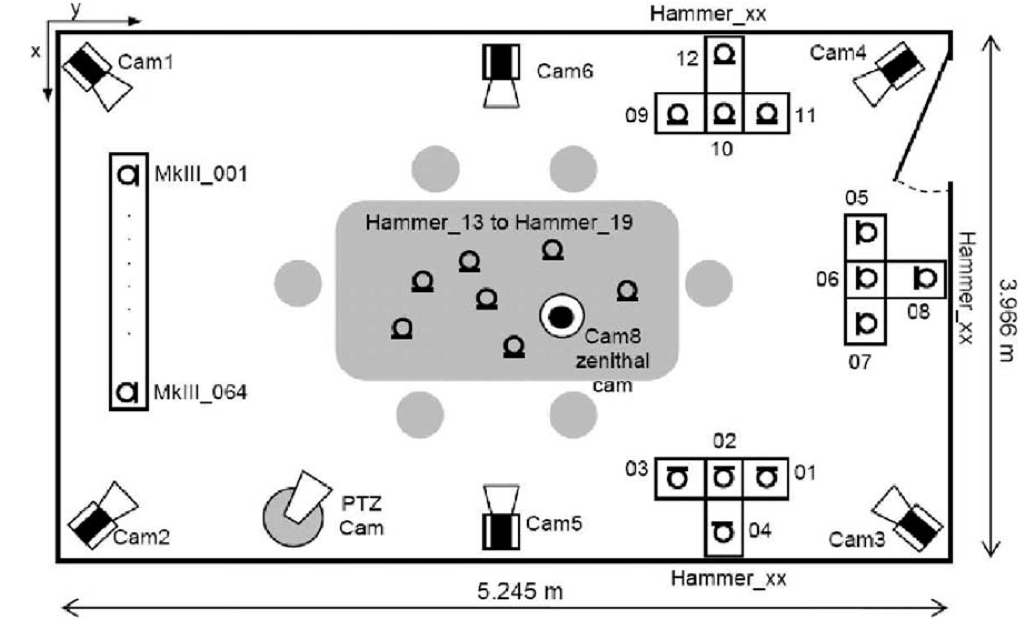
\includegraphics[scale=0.4]{figuras/3.TrabalhosCorrelatos/upc.png}
		\end{center}
		\caption{A configuração do ambiente inteligente UPC~\cite{salah}.}
		\label{upc}
	\end{figure}

Os sensores utilizados e as condições do ambiente inteligente UPC deste projeto são descritos pela Figura \ref{upc}. Os seguintes sensores foram utilizados:

	\begin{itemize}
		\item quatro câmeras nos cantos da sala (rotuladas como Cam1 a Cam4 na Figura \ref{upc});
		\item uma câmera \textit{zenithal fish-eye} no telhado (rotulada como Cam8 na Figura \ref{upc});
		\item uma câmera ativa apontada e com zoom para a porta de entrada para capturar as faces das pessoas que entram na sala (rotulada como PTZ na Figura \ref{upc});
		\item um \textit{array} de microfones NIST Mark III de 64 canais ;
		\item três \textit{clusters} de microfone de 4 canais no formato de T;
		\item oito microfones no teto;
	\end{itemize}


\begin{figure}[hbt]
		\begin{center}
			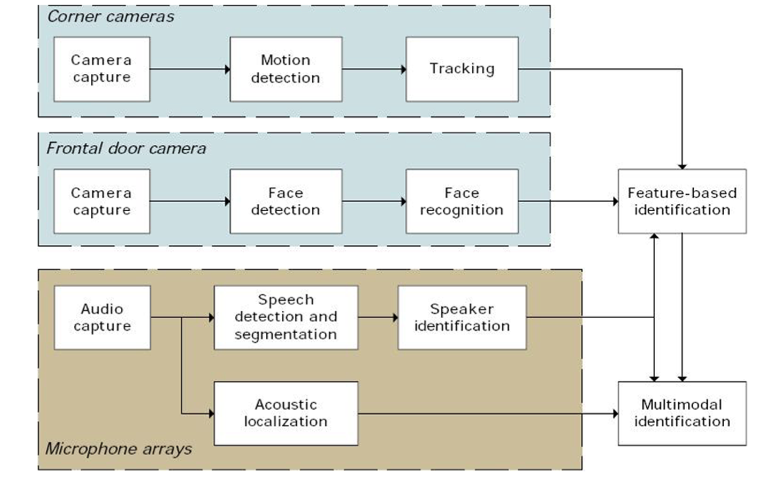
\includegraphics[scale=0.5]{figuras/3.TrabalhosCorrelatos/workflow.png}
		\end{center}
		\caption{\textit{Workflow} da informação na arquitetura do ambiente inteligente UPC~\cite{salah}.}
		\label{workflow}
	\end{figure}

As imagens coletadas pelas câmeras no sistema são utilizadas para detecção de movimento, rastreamento, detecção e reconhecimento facial e serão analisadas a seguir. Como mencionado, o sistema do projeto também promove localização dos usuários no ambiente, porém utiliza amostras de áudio como dados de entrada e por isso não será analisado.

\subsection{Detecção de movimento e Rastreamento}

A detecção de movimento utilizada tenta separar o ``primeiro plano'' do ``fundo'' para o seu funcionamento. O método que o projeto utiliza é baseado na detecção de objetos em movimento sob a suposição que imagens em uma cena sem objetos em movimento mostra regularidades, que podem ser modeladas utilizando métodos estáticos. O conjunto de treinamento é construído por sequências pequenas de gravações \textit{offline} feitas da sala vazia.

Para realizar o rastreamento foi utilizado a abordagem de um mapa de ocupação probabilística (\textit{probabilistic occupancy map} - POM)~\cite{pom} simplificado para ambientes internos, onde as trajetórias de movimentos são curtas e menos frequentes quando comparadas com trajetórias em ambientes externos. Somente as quatro câmeras nos cantos são utilizadas.

Nesta abordagem, o mapa de ocupação é utilizado para projetar a imagem de um esboço de uma pessoa (um retângulo simples) em cada visão das câmeras.  As sobreposições entre os esboços e as detecções de movimento na imagem entre as várias câmeras indicam a presença de uma pessoa. A Figura~\ref{fig:pom} ilustra a distribuição da probabilidade de ocupação produzida pelo algoritmo. 

\begin{figure}[hbt]
		\begin{center}
			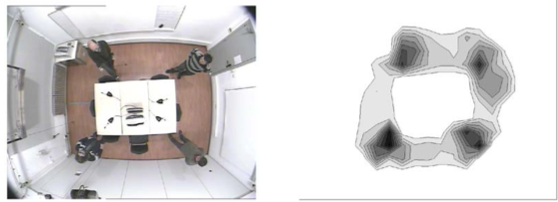
\includegraphics[scale=0.5]{figuras/3.TrabalhosCorrelatos/pom.png}
		\end{center}
		\caption{Mapa de ocupação probabilística. Adaptada de~\cite{salah}.}
		\label{fig:pom}
	\end{figure}

\subsection{Detecção e Reconhecimento Facial}

A detecção de face utilizada no projeto é realizada utilizando o método \textit{Viola-Jones}~\ref{ref:viola-jones} utilizando a biblioteca \textit{OpenCV}. Somente a câmera que está apontada para a porta é utilizada, pois esta é a única que fornece imagens em uma qualidade necessária. As outras câmeras, fornecem imagens em baixa resolução e pequenas demais.  

O módulo de detecção, pela maneira que foi projetado, só detecta faces frontais, em que os dois olhos, o nariz e a boca são visíveis. Como resultado da detecção de face, é retornada uma imagem contendo uma caixa delimitadora da face detectada.

O reconhecimento facial no ambiente inteligente UPC é realizado utilizando uma técnica que aproveita a vantagem que o ambiente é constantemente monitorado e combina a informação de várias imagens para realizar o reconhecimento.  Imagens que são fornecidas pelo módulo de detecção.

Para cada sequência de imagens, as faces de um mesmo indivíduo são agrupadas. Então, para cada grupo, o sistema compara as imagens com a galeria de imagens. Para cada grupo de imagens, as decisões individuais são combinadas em uma decisão única para o grupo.

Uma abordagem baseada em PCA (\textit{Principal Component Analisys}) foi utilizada para comparação entre as imagens, pois possui a menor complexidade computacional necessária para aplicações em tempo real~\cite{salah}.

%%%%%%%%%%%%%%%%%%%%%%%%%%%%%%%%%%%%%%%%%%%%%%%%%%%%%%%%%%%%%%%%%%%%%%%%%%%%%%%%%%%%%%%%%%%%%%%%%%%%%%%%%%%%%%%%%%%%%%%%%%%%%%%%%%%%%%%%%%%%%%%%%%%%%%%%%%%%%%%%%%%%%%%%%%%%%%%%%%%%%%%%%%%%%%%%%%%%%%%%%%%%%%%%%%%%%%%%%%%%%%%%%%%%%%%%%%%%%%%%%%%%%%%%%%%%%%%%%%%%%%%%%%%%%%

\section{Projeto DIVA}

Esse projeto~\cite{trivedi} foi apelidado de Projeto DIVA pois nele foi desenvolvido uma nova arquitetura para ambientes inteligentes chamado DIVA. Ele apresenta detalhes de um projeto de pesquisa de longo prazo, onde ambientes inteligentes com funcionalidades úteis são projetados, construídos e avaliados sistematicamente. 

Esta nova arquitetura pode ser vista como uma rede inteligente e ativa de câmeras, onde várias câmeras são controladas para prover uma ampla gama de funcionalidades. Algumas destas incluem detecção de intrusos, rastreamento várias pessoas, pose do corpo e análise de postura, identificação de pessoas, modelagem do corpo humano e análise do movimento.

O sistema proposto pelo Projeto DIVA monitora o ambiente em baixa resolução de forma contínua, detectando somente a presença e suas dimensões. Formas de aquisição de imagens mais detalhadas são ativadas quando um evento ou atividade de potencial interesse é detectado. Esses eventos serão os focos de atenção do sistema.

O monitoramento de baixa resolução e de grande área do ambiente é alcançado graças a algumas câmeras de amplo ângulo de visão e estáticas. Com um pequeno número de câmeras PTZ (\textit{pan/tilt/zoom}) ativas, múltiplos focos de atenção podem ser mantidos de forma simultânea.

	\begin{figure}[hbt]
		\begin{center}
	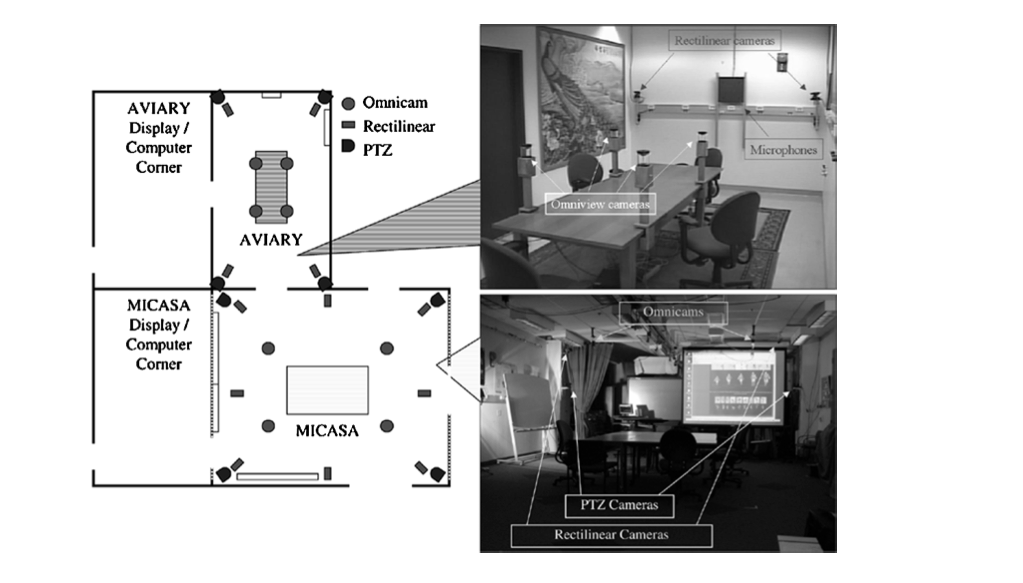
\includegraphics[scale=0.5]{figuras/3.TrabalhosCorrelatos/micasa_aviary.png}
		\end{center}
		\caption{Representação dos ambientes inteligentes MICASA e AVIARY~\cite{trivedi}.}
		\label{micasa_aviary}
	\end{figure}

O Projeto DIVA possui dois ambientes inteligentes separados, mas conectados. O primeiro é chamado de AVIARY foi projetado para ser uma pequena sala de conferências. O segundo chamado de MICASA foi projetado para ser uma pequena sala de aula. A Figura~\ref{micasa_aviary} mostra fotos dos dois ambientes e como estão conectados, além da disposição dos sensores utilizados.

Os sensores no ambiente inteligente AVIARY incluem:

	\begin{itemize}
		\item uma rede de quatro câmeras omnidirecionais;
		\item quatro câmeras PTZ;
		\item quatro câmeras retilíneas estáticas;
		\item dois \textit{arrays} de microfones com quatro microfones cada;
	\end{itemize}

As quatro câmeras omnidirecionais (ODVSs) estão perto dos cantos de uma mesa de reunião, cobrindo o quarto inteiro de dentro para fora, como mostrado na Figura \ref{micasa_aviary}. As câmeras PTZ e retilíneas estão nos ``vértices'' da sala a $\displaysytle 1.4m$ acima do chão. Os dois \textit{arrays} de microfones foram instalados na parede e no teto.

% Um computador é alocado para rastreamento, utilizando imagens das quatro câmeras omnidirecionais ou imagens das quatro câmeras retilíneas estáticas. Outro computador é utilizado para analisar os eventos de áudio e de vídeo. Um terceiro computador é utilizado para arquivar \textit{streams} de áudio e vídeo para posterior recuperação.

O ambiente inteligente MICASA é duas vezes maior que o AVIARY. Os sensores utilizados são:
	
	\begin{itemize}
		\item uma rede de quatro câmeras omnidirecionais;
		\item quatro câmeras PTZ;
		\item oito câmeras retilíneas estáticas;
	\end{itemize}

As câmeras omnidirecionais são instaladas no teto, como mostrado na Figura \ref{micasa_aviary}. As câmeras PTZ e quatro câmeras retilíneas foram instaladas de maneira similar ao ambiente AVIARY. As quatro câmeras retilíneas restantes foram instaladas nas paredes como mostrado como mostrado na Figura \ref{micasa_aviary}. As câmeras nos vértices possuem maior campo de visão para cobrir toda a sala e fazem parte do array de câmeras para rastreamento.

\subsection{Rastreamento e Reconhecimento facial}
 
No Projeto DIVA foi desenvolvido um sistema em tempo-real que utiliza a rede de câmeras omnidirecionais e é responsável pelo rastreamento e reconhecimento facial. 

O rastreamento é feito utilizando subtração do fundo~\ref{sec:deteccao-objeto} com remoção de sombras para detectar as silhuetas dos novos usuários no ambiente.  Com isso, essas silhuetas são rastreadas imagem por imagem~\ref{sec:rastreamento}.

Os resultados do rastreamento são utilizados para controlar o reconhecimento facial. As imagens obtidas do rastreamento são processadas utilizando um método de segmentação de tom de pele e são recortadas para obter as imagens com possíveis faces. 

Essas imagens, então, são classificadas para rejeitar as imagens sem faces. Para essa classificação é utilizado o método \textit{Eigenfaces}~\ref{sec:reconhecimento}. Este último também é utilizado para realizar o reconhecimento facial utilizando a classificação do ``vizinho'' mais príximo.

O treinamento do algoritmo \textit{Eigenfaces} implementado no sistema do Projeto DIVA é feito utilizando um banco com $\displaystyle 200$ imagens de faces de várias pessoas diferentes.

	\begin{figure}[hbt]
		\begin{center}
			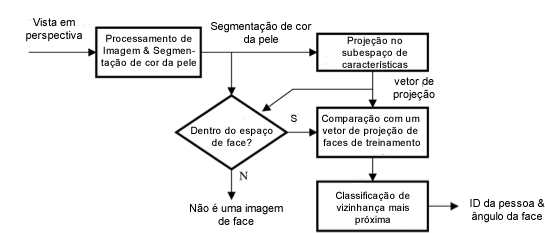
\includegraphics[scale=0.8]{figuras/3.TrabalhosCorrelatos/facerec.png}
		\end{center}
		\caption{Método de detecção e reconhecimento facial~\cite{trivedi}.}
		\label{facerec}
	\end{figure}


\chapter{Sistema \textit{True}}

Observando a realidade de um ambiente inteligente fica claro que as informações como posição das pessoas e suas respectivas identidades são imprescindíveis para que decisões possam ser tomadas. Atualmente, a maioria das soluções encontradas para fornecer esse tipo de informação foram projetadas para funcionar em ambientes rigidamente definidos. Com isso, não seria adequado tentar incorporar soluções como estas em um ambiente com diferentes dimensões, condições de iluminação, posição dos móveis, diferentes sensores pois este resultaria em um cenário diferente. Além disso, a solução deve ser integrada com o middleware \textit{UbiquitOS}, o qual gerência os serviços providos pelo ambiente inteligente.

Esse trabalho propõe, então, um sistema aberto de rastreamento, localização e identificação de pessoas em um ambiente inteligente integrado com o middleware \textit{UbiquitOS}. Tal sistema será chamado de TRUE, \textit{\textbf{T}racking and \textbf{R}ecognizing \textbf{U}sers in the \textbf{E}nvironment}.

O Sistema \textit{True} é um sistema monomodal que utiliza somente dados visuais, como imagens de cor e profundidade. As imagens de profundidade serão utilizadas no rastreamento e localização dos usuários no ambiente, e as imagens de cor serão utilizadas no reconhecimento facial e no cadastro dos usuários. Portanto, os dispositivos presentes no ambiente devem ser capazes de fornecer esses tipos de dados a um taxa e qualidade adequada. 

Para obter os dados necessários, o sistema utiliza o sensor \textit{Kinect} da Microsoft descrito no Apêndice~\ref{sec:kinect}, um dispositivo bastante acessível e capaz de fornecer imagens de cor e de profundidade sincronizadas a uma taxa e qualidade necessária.

O sistema \textit{True} é dividido em quatro módulos principais:


	\begin{itemize}
		\item \textbf{Módulo de Rastreamento e Localização}: parte do sistema responsável pelo rastreamento e localização dos usuários no ambiente.
		\item \textbf{Módulo de Reconhecimento}: parte do sistema responsável por identificar os usuários rastreados.
		\item \textbf{Módulo de Registro}: parte do sistema responsável pelo cadastro de novos usuários e treino do sistema.
		\item \textbf{Módulo \textit{UbiquitOS}}: parte do sistema responsável pela integração e comunicação do sistema com o middleware.
	\end{itemize}

O Módulo de Registro é independente dos demais. Porém, os outros dois módulos devem trocar informações entre si para centralizar todas as informações (localização e reconhecimento) de todos usuários rastreados no ambiente. A seguir, é explicado mais detalhadamente cada módulo e como tal troca de informações ocorre.



	\section{Módulo de Reconhecimento}

	O Módulo de Reconhecimento é responsável pela identificação dos usuários no ambiente utilizando a face como característica biométrica. A face foi escolhida por permitir um reconhecimento não intrusivo, como mencionado na Seção~\ref{sec:biometria}. A detecção e o reconhecimento são feitos a partir de imagens de usuários que são repassadas pelo Módulo de Rastreamento. Estas imagens são compostas somente pela região em que o usuário se encontra, como mostrado na Figura~\ref{fig:users-img}.

	Basicamente, o processo de reconhecimento é realizado pelas seguintes etapas (Figura~\ref{fig:processo-reconhecimento}):

		\begin{figure}[htb]
			\begin{center}
				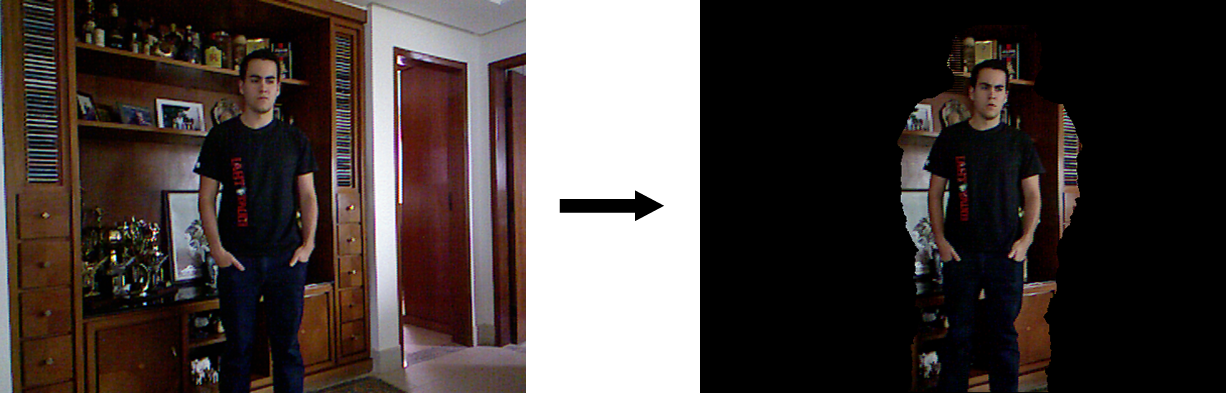
\includegraphics[scale=0.3]{figuras/4.ProblemaEProposta/users-img.png}
			\end{center}
			\caption{Exemplo de uma imagem composta somente pela região em que o usuário se encontra.}
			\label{fig:users-img}
		\end{figure}

		\begin{enumerate}
			\item Obtenção da imagem de entrada composta somente pelo usuário cujo reconhecimento foi requisitado.
			\item Pré-processamento da imagem, ou seja, conversão da imagem em escala de cinza.
			\item Detecção facial na imagem. Caso nenhuma face seja encontrada, retorna ``vazio''. Observa-se que no máximo uma face pode ser encontrada nesta imagem.
			\item Processamento da imagem: uma nova imagem é criada recortando a região da face encontrada. A imagem é, então, redimensionada e equalizada criando assim um padrão de tamanho, brilho e contraste aumentando a acurácia do reconhecimento.
			\item Reconhecimento facial com a técnica \textit{Eigenfaces}.
			\item Retorno do nome do usuário com a face ``mais parecida'' e a confiança do reconhecimento.
		\end{enumerate}

		\begin{figure}[htb]
			\begin{center}
				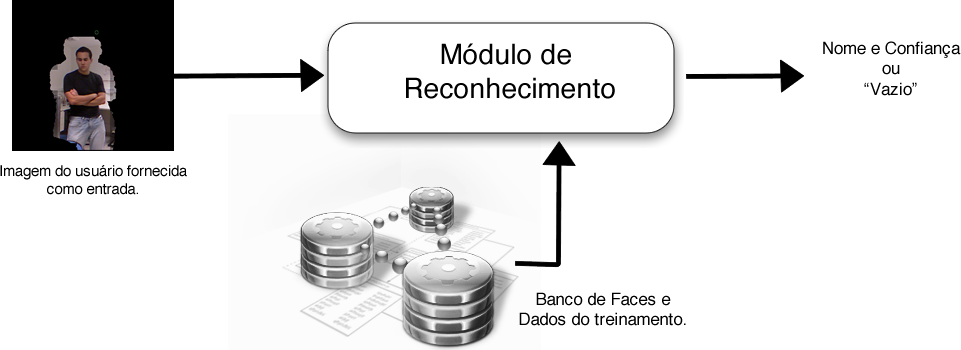
\includegraphics[scale=2.0]{figuras/4.ProblemaEProposta/reconhecimento-simples.png}
			\end{center}
			\caption{Módulo de Reconhecimento do Sistema TRUE.}
			\label{fig:processo-reconhecimento}
		\end{figure}

	% O Módulo de Reconhecimento é dependente do de Rastreamento. Ele ficará ocioso
	% até que chegue uma requisição de reconhecimento de um determinado usuário. A
	% Seção~\ref{sec:rastreamento-reconhecimento} explica mais detalhadamente a
	% relação entre os dois módulos.

	A seguir serão relatados as etapas de Pré-processamento e Processamento da imagem. Depois, serão apresentados em detalhes as etapas de Detecção e Reconhecimento facial.

	\subsection{Pré-processamento e Processamento da Imagem}
		
		As etapas de pré-processamento e processamento das imagens (etapas 2 e 4 mencionadas acima) permitem criar um padrão nas mesmas aumentando a acurácia do reconhecimento. No Sistema TRUE estas etapas consistem em converter a imagem em escala de cinza, recortá-la, redimensioná-la e equalizá-la, criando, assim, padrões de cor, tamanho, brilho e contraste.

		A Figura~\ref{fig:greyscale} exemplifica uma imagem capturada de uma face, a mesma convertida em escala de cinza e depois equalizada. O
		Apêndice~\ref{apend:processamento} contém trechos de código em linguagem C que implementam tais etapas.

		\begin{figure}[htb]
			\begin{center}
				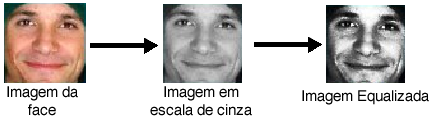
\includegraphics[scale=0.7]{figuras/4.ProblemaEProposta/greyscale.png}
			\end{center}
			\caption{Exemplo de uma imagem de face capturada, a mesma em escala de cinza e depois equalizada. Adaptada de~\cite{shervin}.}
			\label{fig:greyscale}
		\end{figure}

	\subsection{Detecção Facial}

		A detecção facial (etapa 3 mencionada acima) foi desenvolvida utilizando o método \textit{Viola-Jones} apresentado na Seção~\ref{ref:viola-jones}. Este método é adequado para construir uma abordagem de detecção facial rápida e eficaz~\cite{violajones} em tempo real. Além disso, o \textit{Viola-Jones} é implementado pela biblioteca \textit{OpenCV}~\cite{opencv_library} (\textit{Open Source Computer Vision}). Basicamente, o processo de detecção facial procura por uma face em uma imagem pré-processada. Para realizar detecção facial utilizando o método \textit{Viola-Jones} é necessário a utilização de um classificador em cascata, como mencionado na Seção~\ref{subsec:reconhecimento}. Portanto, entre os diversos classificadores em cascata presentes na biblioteca \textit{OpenCV}, o Sistema TRUE utiliza o classificador \textit{haarcascade\underline{ }frontalface\underline{ }alt.xml}, um classificador treinado para detectar faces frontais em imagens.

		% A Figura~\ref{fig:diagrama-deteccao} mostra o fluxo básico do processo de detecção de faces no Sistema TRUE.
		% 	\begin{figure}[H]
		% 	\begin{center}
		% 		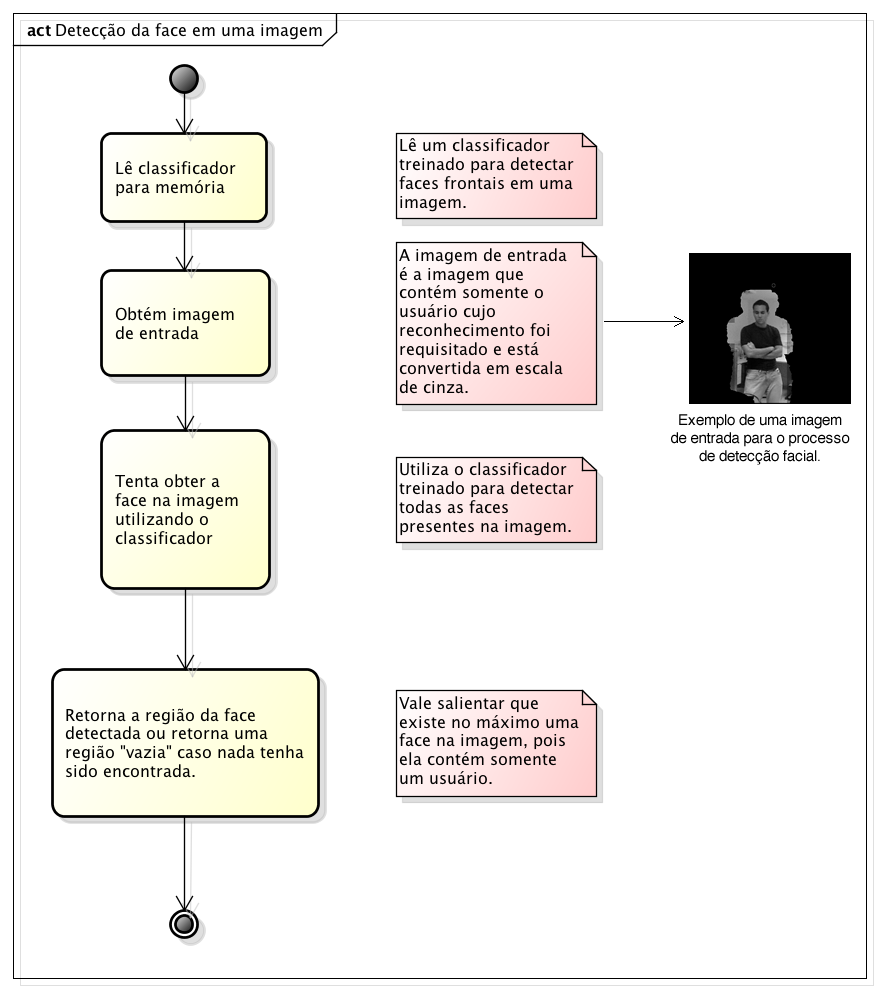
\includegraphics[scale=0.5]{figuras/4.ProblemaEProposta/diagrama-detectar-face.png}
		% 	\end{center}
		% 	\caption{Fluxo de execução do processo de detecção facial no Sistema TRUE.}
		% 	\label{fig:diagrama-deteccao}
		% \end{figure}

		O processo de básico de detecção de faces no Sistema TRUE possui as seguintes etapas:

		\begin{enumerate}
			\item Leitura de um classificador treinado para detectar faces em uma image.
			\item Obtenção da imagem de entrada (esta imagem é composta somente pelo usuário e esta na escala de cinza).
			\item Detecção da face na imagem utilizando o classificador.
			\item Retorno da região da face detectada ou retorno ``vazio'' caso nenhuma face tenha sido encontrada. Observa-se que existe no máximo uma face na imagem, pois contém somente um usuário.
		\end{enumerate}

	\subsection{Reconhecimento Facial com \textit{Eigenfaces}}

		A etapa do reconhecimento facial propriamente dito, correspondente a etapa 5 mencionada acima, foi desenvolvida utilizando a técnica \textit{Eigenfaces} (Seção~\ref{sec:reconhecimento}). Esta técnica consiste em uma técnica bastante satisfatória quando utilizada sobre uma base de faces relativamente grande, permitindo ao sistema inferir, das imagens das faces suas principais características e, partindo delas, realizar o reconhecimento facial utilizando um número reduzido de cálculos~\cite{artigo-eigenface}, permitindo, assim, um reconhecimento em tempo real.

		A base de dados utilizada no Sistema TRUE é formada por imagens no formato PGM (\textit{Portable Gray Map}) com tamanho de 92x112 pixels e em escala de cinza. A base é composta por um banco de faces de alunos voluntários de Ciência da Computação da Universidade de Brasília e por um banco de imagens de faces da Universidade de Cambridge~\cite{cambridgeFaceDb}, mostrado na Figura~\ref{fig:cambridgeFaceDb}. Este último, é formado por imagens de faces de 40 pessoas diferentes. Para cada pessoa, existem 10 diferentes imagens obtidas em diferentes momentos, com diferentes condições de iluminação, diferentes expressões faciais (olhos abertos e fechados, sorrindo e não sorrindo, entre outros) e diferentes detalhes faciais (com e sem óculos). 

		\begin{figure}[H]
			\begin{center}
				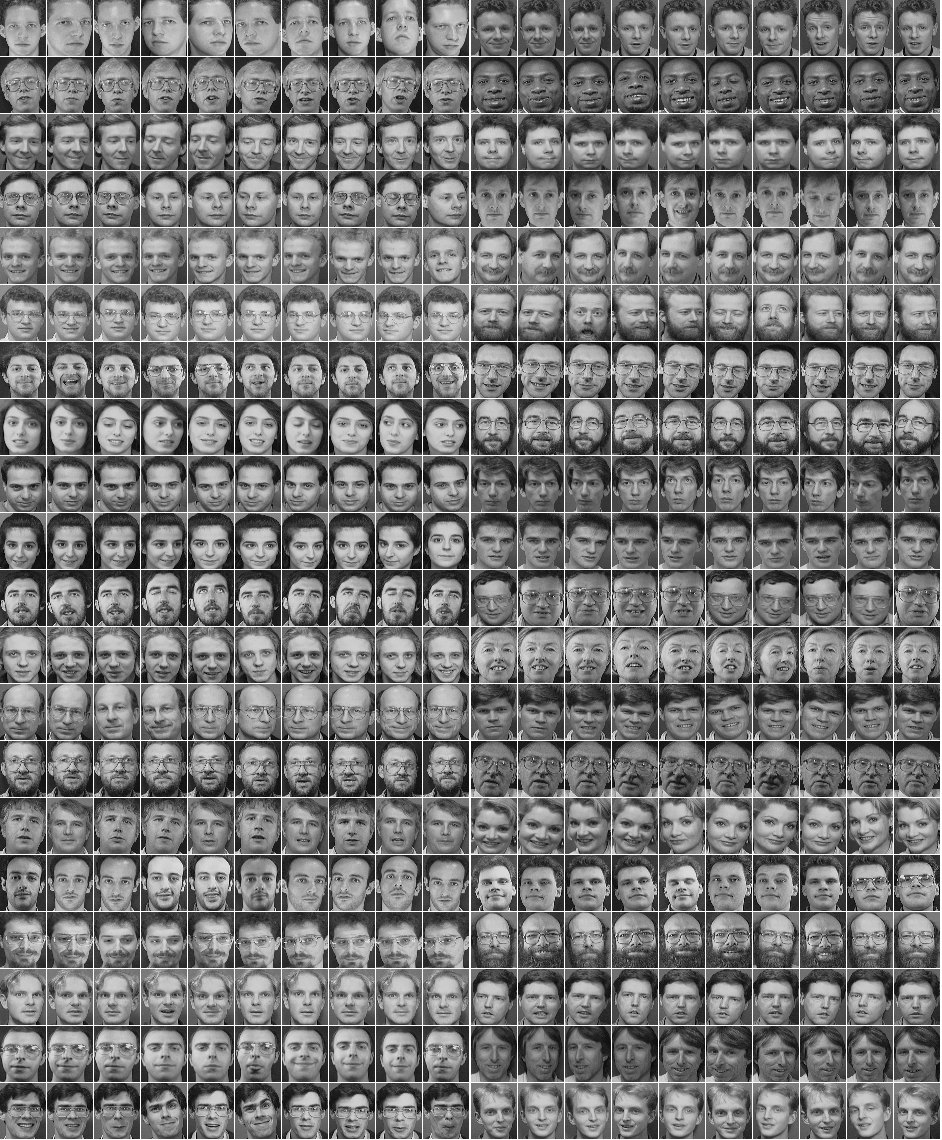
\includegraphics[scale=0.3]{figuras/4.ProblemaEProposta/cambrigdefacedb.png}
			\end{center}
			\caption{Banco de imagens de faces da Universidade de Cambridge~\cite{cambridgeFaceDb}.}
			\label{fig:cambridgeFaceDb}
		\end{figure}

		A Figura~\ref{fig:diagrama-reconhecimento} mostra o fluxo básico do processo de reconhecimento facial no Sistema TRUE.

			\begin{figure}[htb]
			\begin{center}
				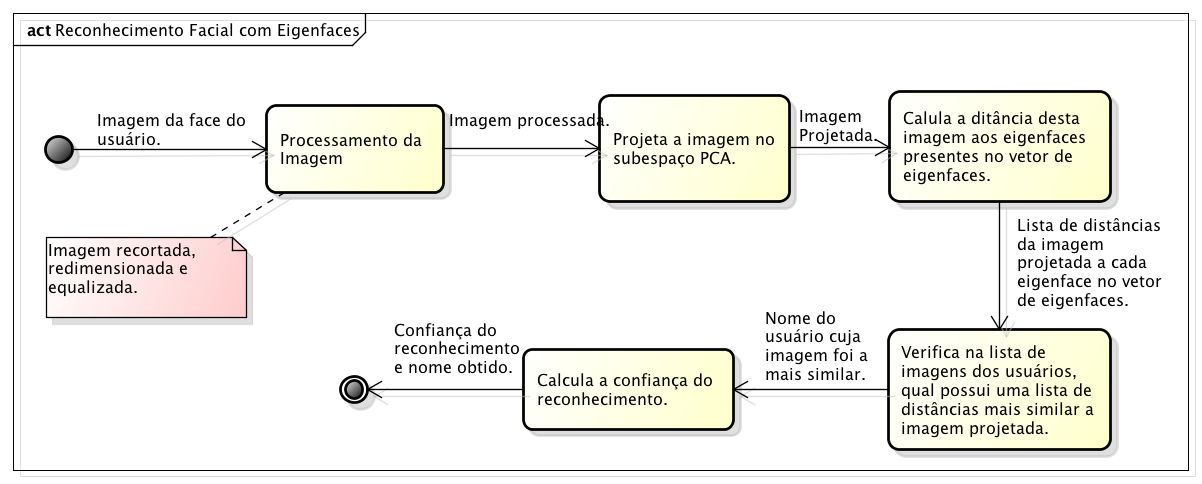
\includegraphics[scale=0.5]{figuras/4.ProblemaEProposta/diagrama-reconhecimento2.png}
			\end{center}
			\caption{Fluxo de execução do processo de reconhecimento facial no Sistema TRUE.}
			\label{fig:diagrama-reconhecimento}
		\end{figure}

		% A primeira etapa consiste na leitura dos dados de treinamento. Esses dados são compostos pela lista dos nomes e imagens das faces dos usuários cadastrados no sistema, pelo vetor de \textit{Eigenfaces}, pela \textit{Eigenface} média e pelos \textit{eigenvalues}.

		% Uma das etapas intermediárias consiste no cálculo da distância entre a imagem projetada no subespaço PCA aos eigenfaces. Inicialmente, o cálculo desta distância era feito utilizando distância euclidiana, porém não apresentava bons resultados em algumas condições. Portanto, este cálculo passou a ser feito utilizando distância Mahalanobis. Contudo, ela também não apresentou bons resultados em alguns casos. Então, alguns testes foram feitos utilizando as duas distâncias de maneira conjunta: uma imagem só é tida como reconhecida quando o resultado das duas distâncias apontarem para a mesma identidade. Com isso, houve uma melhora significativa dos resultados.

		Uma das etapas intermediárias consiste no cálculo da distância entre a imagem projetada no subespaço PCA aos \textit{eigenfaces}. Inicialmente, o cálculo desta distância era feito utilizando distância Euclidiana. Contudo, testes foram realizados com alguns usuários, em que o sistema realizava 20 tentativas de reconhecimento de usuários, e os resultados não foram satisfatórios. Portanto, os mesmos testes foram realizados utilizando distância Mahalanobis. Porém, os resultados também não foram satisfatórios. Então, os mesmos testes foram feitos utilizando as duas distâncias de maneira conjunta: uma imagem só é tida como reconhecida quando o resultado das duas distâncias apontarem para a mesma identidade. Com isso, houve uma melhora significativa dos resultados. Os resultados destes testes são mostrados na Tabela~\ref{tab:distancias}, onde fica claro a melhora dos resultados quando se utiliza ambas distâncias. Nessa tabela, os nome Pessoa1, Pessoa2, Pessoa3, são nomes dados as pessoas cujas fotos estão presentes no banco de imagens de faces da Universidade de Cambrige~\cite{cambridgeFaceDb}.

		\begin{table}[H]
		\begin{center}
			\caption{Resultados do teste de reconhecimento feito com o usuário Danilo utilizando as diferentes distâncias.}
			\label{tab:distancias}
			\begin{tabular}{|c|c|c|c|c|c|c|c|}
				\hline & \bf \begin{sideways}Danilo\end{sideways} & \bf \begin{sideways}Pedro\end{sideways} & \bf \begin{sideways}Ana\end{sideways} & \bf \begin{sideways}Pessoa1\end{sideways} & \bf \begin{sideways}Pessoa2\end{sideways} & \bf \begin{sideways}Pessoa3\end{sideways} & \bf \begin{sideways}Desconhecido\end{sideways}\\
				\hline \bf Euclidiana & 45\% & 40\% & & 5\% & 5\% & 5\% &\\
				\hline \bf Mahalanobis & 40\% & & 15\% & 35\% & 10\% & &\\
				\hline \bf Ambas Distâncias & 75\% & & & & & & 25\%\\
				\hline
			\end{tabular}
		\end{center}
	\end{table}

		A última etapa consiste no cálculo da confiança do reconhecimento. Este cálculo foi feito utilizando a distância da imagem de entrada do usuário à imagem mais similar das imagens de treinamento. O valor da confiança varia de 0.0 a 1.0, em que uma confiança de 1.0 significaria uma ``correspondência perfeita''. A fórmula utilizada para calcular a confiança é uma métrica muito básica que não necessessariamente é muito real, dada pela Fórmula~\ref{eq:confianca}~\cite{shervin}. Nesta fórmula $\displaystyle d_e$ é a distância da imagem de entrada do usuário a imagem mais similar das imagens de treinamento, $\displaystyle n_t$ é o número de imagens utilizadas no treinamento e $\displaystyle n_e$ é o número de \textit{eigenfaces}.


		\begin{equation}
			\label{eq:confianca}
			Confianca = 1 - \frac{\sqrt{\frac{d_e}{n_t * n_e}}}{255}
		\end{equation}






















	\section{Módulo de Rastreamento}

	O Módulo de Rastreamento será responsável por rastrear os usuários no ambiente inteligente, determinar a sua localização física em relação ao \textit{Kinect} e gerenciar suas identidades. Para realizar o rastreamento e localização dos usuários é utilizado a biblioteca \textit{OpenNI} (\textit{Open Natural Interaction}). Trata-se de um \textit{framework} que define \textit{APIs} para o desenvolvimento de aplicações de interação natural. Utilizando as imagens de profundidade, a detecção e o rastreamento são feito utilizando subtração de fundo, descrito na Seção~\ref{sec:deteccao-objeto}, e os objetos detectados são representados por suas silhuetas, descrita na Seção~\ref{sec:representacao-objeto}.

	As imagens utilizadas para o rastreamento são imagens de profundidade, exemplificada na Figura~\ref{fig:depthmaps}, providas pelo \textit{Kinect} que são obtidas utilizando o método de Luz Estruturada descrito na Seção~\ref{sec:luz-estruturada}. Tais imagens de profundidade nada mais são que \textit{depth maps} (mapas de profundidade), em que cada pixel da imagem contém o valor estimado da distância em relação ao sensor. O \textit{Kinect} fornece esses dados a uma taxa de $\displaystyle 30 fps$ (\textit{frames} por segundo) com uma resolução $\displaystyle 640px$ x $\displaystyle 480px$.
	

	\begin{figure}[H]
		\begin{center}
			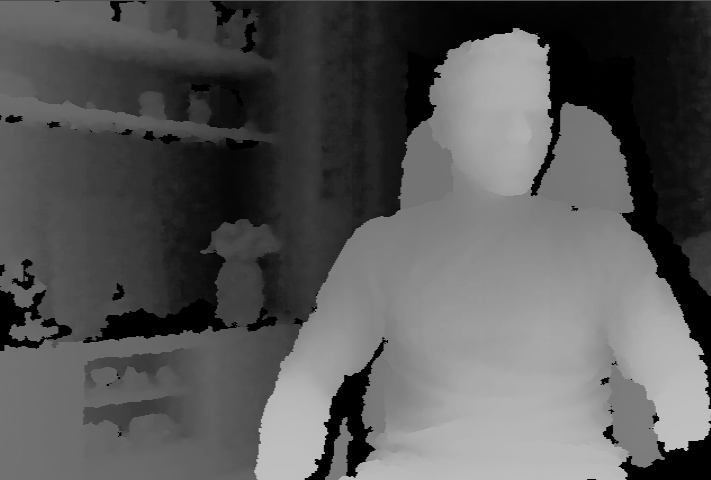
\includegraphics[scale=0.45]{figuras/4.ProblemaEProposta/mapa-profundidade.png}
		\end{center}
		\caption{Exemplo de uma imagem de profundidade fornecida pelo \textit{Kinect}.}
		\label{fig:depthmaps}
	\end{figure}

	Utilizando os mapas de profundidade é possivel calcular as coodernadas $\displaystle (x,y,z)$, em relação ao sensor, de qualquer pixel da imagem. Dessa forma, a posição de um usuário rastreado é determinada utilizando as coordenadas presentes no pixel que representa seu centro geométrico. Sendo assim ao fixar a posição do \textit{Kinect} no ambiente, conseguiremos estimar a localização de qualquer usuário rastreado em tempo real. A Figura~\ref{fig:localizacao} mostra um usuário rastreado pelo Sistema TRUE onde suas coordenadas em relação ao \textit{Kinect} foram estimadas utilizando os valores de profundidade referente ao pixel que representa seu centro de massa geométrico. Os valores das coordenadas $\displaystle (x,y,z)$ estão milimetros.

	\begin{figure}[H]
		\begin{center}
			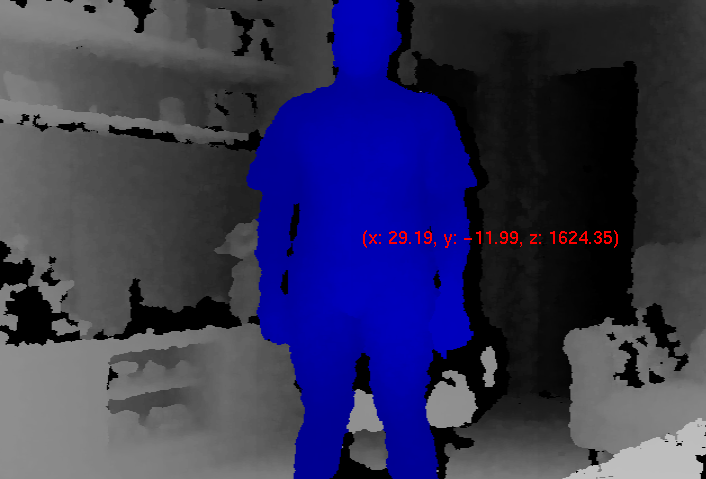
\includegraphics[scale=0.45]{figuras/4.ProblemaEProposta/localizacao.png}
		\end{center}
		\caption{Imagem do Sistema TRUE de um usuário rastreado e localizado.}
		\label{fig:localizacao}
	\end{figure}
	
	
	\begin{figure}[H]
		\begin{center}
			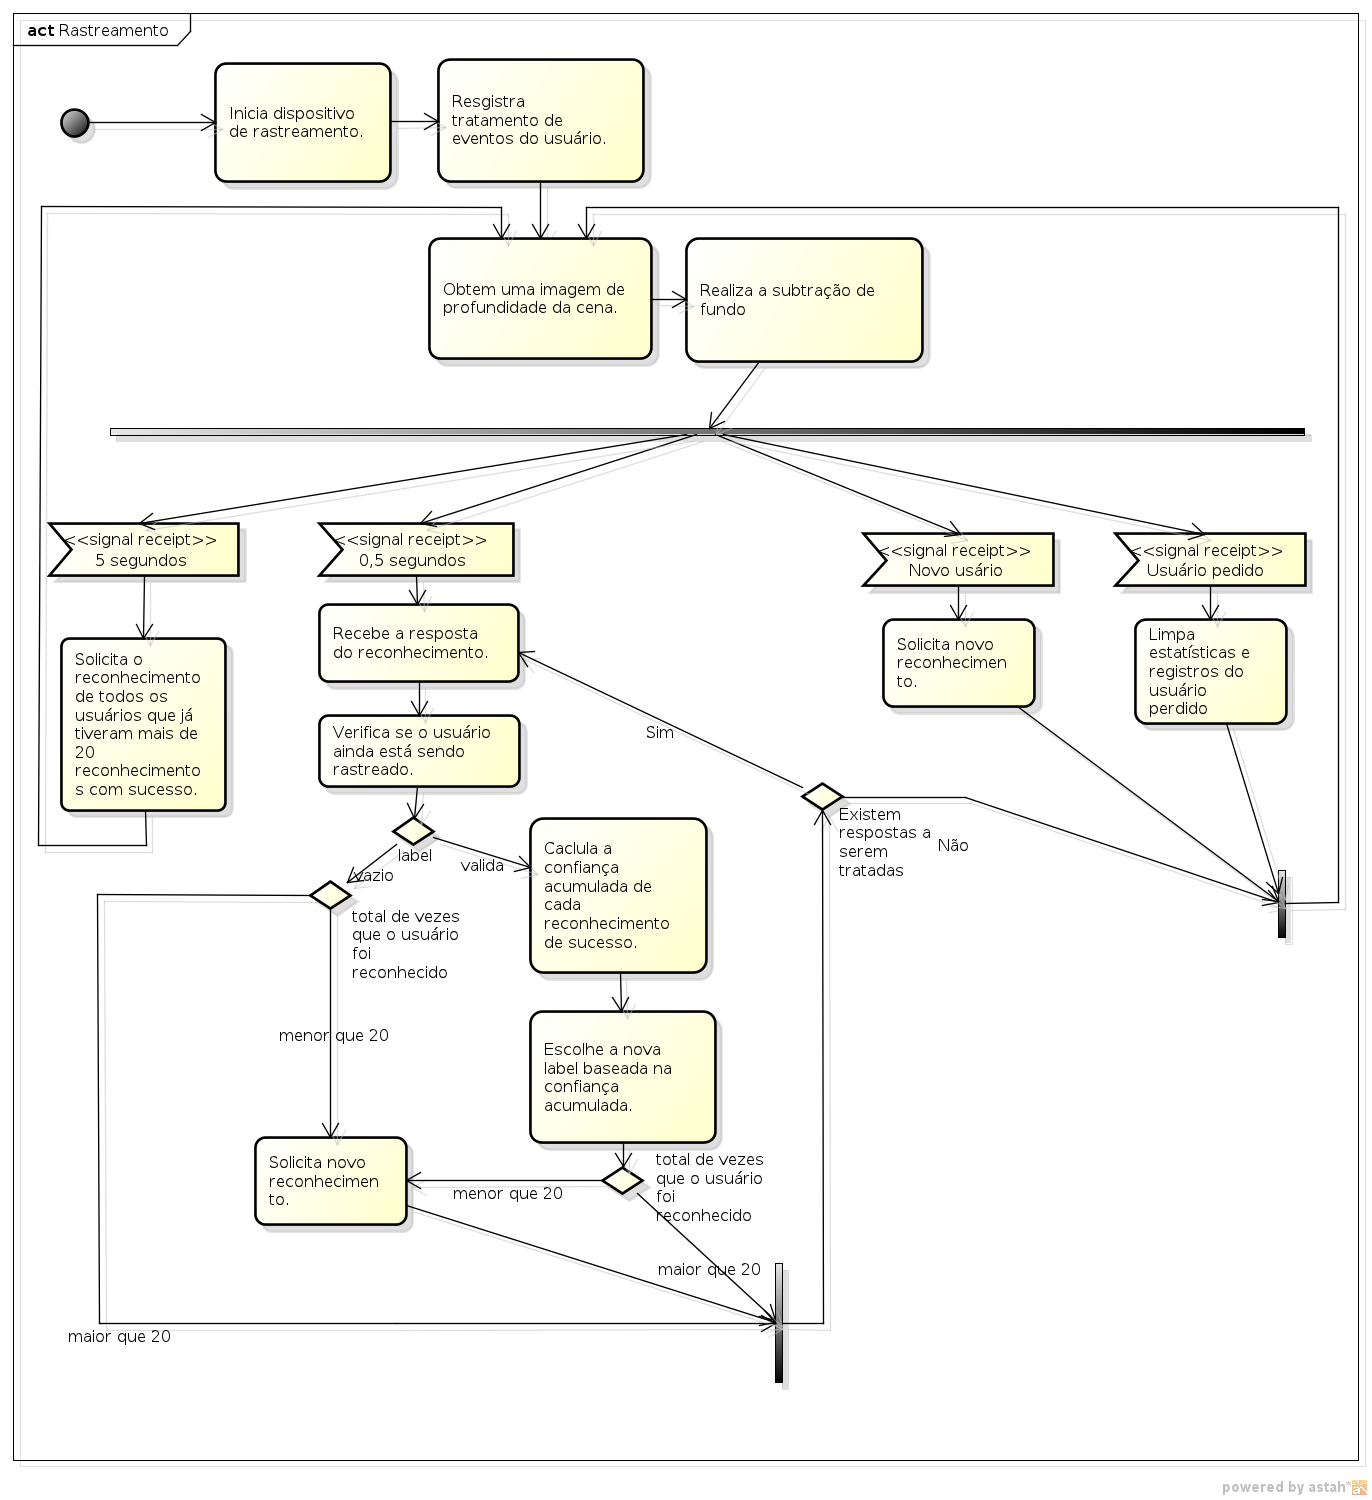
\includegraphics[scale=0.45]{figuras/4.ProblemaEProposta/Rastreamento.png}
		\end{center}
		\caption{Representação das etapas propostas para o rastreamento.}
		\label{fig:processo-rastreamento}
	\end{figure}

	\section{Relação Rastreamento e Reconhecimento}
\label{sec:rastreamento-reconhecimento}

	Até agora, foi mostrado como os Módulos de Rastreamento e de Reconhecimento funcionam de maneira isolada, mas não como se relacionam. O Módulo de Rastreamento detém as informações sobre todos os usuários rastreados no ambiente e é responsável por requisitar reconhecimento ao Módulo de Reconhecimento, que deverá acontecer quando um novo usuário for detectado ou quando for necessário reconhecer um usuário já rastreado.

	Basicamente, quando um novo usuário for detectado, a relação entre rastreamento e reconhecimento acontecerá de acordo com as etapas descritas na Figura~\ref{fig:rastreamento-reconhecimento}.

		\begin{figure}[htb]
			\begin{center}
				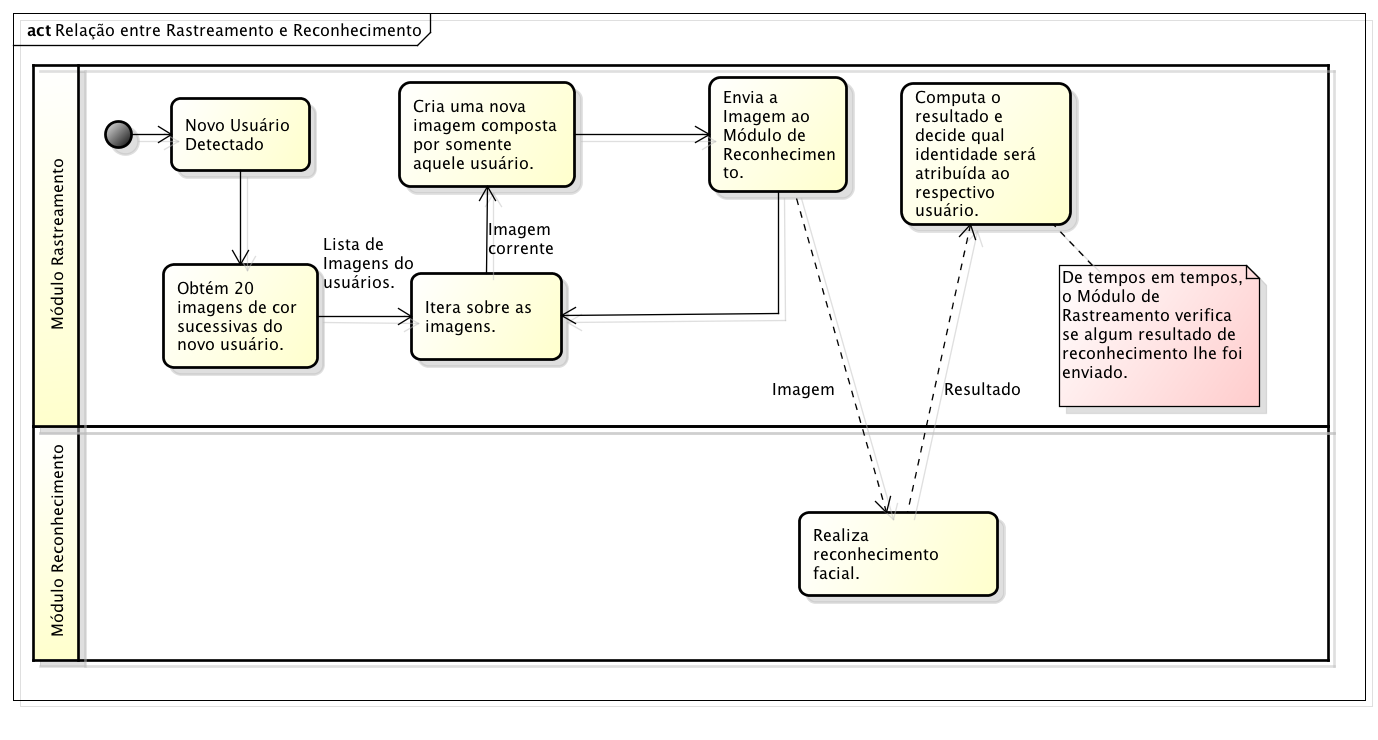
\includegraphics[scale=0.5]{figuras/4.ProblemaEProposta/diagrama-relacao.png}
			\end{center}
			\caption{Representação da relação que o Módulo de Rastreamento terá com o Módulo de Reconhecimento quando um novo usuário for detectado.}
			\label{fig:rastreamento-reconhecimento}
		\end{figure}
	
		% \begin{enumerate}
		%  	\item O Módulo de Rastreamento detecta novo usuário, e obtém um número pré-definido de imagens sucessivas do novo usuário. Para cada imagem, ele cria uma nova imagem de cor contendo somente aquele usuário, como mostrado na Figura (\textbf{colocar a figura aqui}), e a envia para o Módulo de Reconhecimento.
		%  	\item Para cada imagem recebida, o Módulo de Reconhecimento tenta reconhecer o novo usuário e retorna ``vazio'' ou o nome e a confiança do reconhecimento.
		%  	\item O Módulo de Rastreamento verifica se a confiança é maior que um limiar pré-definido, se for ele incrementa o contador que armazena o número de vezes que o usuário foi reconhecido, armazena o nome obtido juntamente com a confiança e calcula qual nome  será atribuído ao novo usuário. Esse cálculo será feito por meio de uma média ponderada utilizando os diferentes resultados obtidos por cada reconhecimento e suas respectivas confianças.
	 % 	\end{enumerate} 
	
	Ao invés de tentar realizar o reconhecimento somente quando novos usuários são detectados, o Sistema TRUE continua a tentar reconhecer os usuários já reconhecidos para melhorar a confiança no reconhecimento. Essas tentativas de reconhecer novamente os usuários ocorrerão em intervalos de tempo pré-definidos seguindo as mesmas etapas de quando um novo usuário for detectado. A única etapa que se difere é a primeira: ao invés de obter várias imagens de um mesmo usuário, são obtidas uma imagem de cada usuário rastreado e as mesmas são enviadas ao Módulo de Reconhecimento.

	Como visto na Figura~\ref{fig:rastreamento-reconhecimento}, ao obter um resultado de reconhecimento para determinado usuário, o Módulo de Rastreamendo deve computar qual identidade será atribuída ao mesmo. Para isso, este módulo mantém para cada usuário o número total de vezes que já foi reconhecido, os diferentes nomes obtidos pelo Módulo de Reconhecimento bem como a confiança média para cada nome e o número de vezes que cada nome foi atribuído ao usuário. Com todos esses dados, a identidade do usuário é escolhida por meio de uma média ponderada entre as confianças de cada nome onde os pesos utilizados são compostos pelo número de vezes que o respectivo nome foi atribuído ao usuário. Vejamos o seguinte exemplo para ilustrar esse cálculo:

	\begin{description}
		Seja João um usuário do ambiente inteligente que está sendo rastreado a algum tempo e que já foi reconhecido algumas vezes. No momento, o Módulo de Rastreamento mantém vários dados sobre o João descritos na Tabela~\ref{tab:joao}. Então, para computar qual identidade será atribuída ao usuário, o Módulo de Rastreamento realiza os cálculos~\ref{eq:joao}. Como o resultado da média ponderada se aproxima mais da confiança do nome João, este foi escolhido como sendo sua identidade.
	\end{description}

	\begin{table}[htb]
		\begin{center}
			\caption{Exemplos de dados de reconhecimento mantidos para cada usuário rastreado pelo Módulo de Rastreamento.}
			\label{tab:joao}
			\begin{tabular}{|c|c|c|}
				\hline \bf Nome & Confiança Média & Número de Vezes \\
				\hline \hline \bf João & 0.947302 & 15 \\
				\hline \bf  Danilo & 0.934010 & 1 \\
				\hline \bf Tales & 0.950320 & 3 \\
				\hline
				\hline \multicolumn{2}{|c|}{\bf Total}  & 19 \\
				\hline
			\end{tabular}
		\end{center}
	\end{table}

	\begin{align}
		\label{eq:joao}
		M_p = \frac{15 * 0.947302 + 1 * 0.934010 + 3 * 0.950320}{19} = 0.947079
	\end{align}

	\begin{align}
	\nonumber & Joao: 0.947079 - 0.947302 = -0.000223\\
		\nonumber & Danilo: 0.934010 - 0.947302 = -0.013292\\
		\nonumber & Tales: 0.950320 - 0.947302 = 0.003018
	\end{align}

	Com todos esses dados de reconhecimento, além dos dados de rastreamento e localização de cada usuário, o Módulo de Rastreamento consegue centralizar todas as informações necessárias de cada usuário. A Figura~\ref{fig:truetotal} exemplifica um usuário rastreado pelo Sistema TRUE onde as informações de localização e identificaçao estão presentes.

	\begin{figure}[htb]
			\begin{center}
				\includegraphics[scale=0.5]{figuras/4.ProblemaEProposta/usuario-identificado.png}
			\end{center}
			\caption{Exemplo de um usuário rastreado e identificado pelo Sistema TRUE.}
			\label{fig:truetotal}
		\end{figure}


	\section{Módulo de Registro}

	O Módulo de Registro será responsável por cadastrar novos usuários no sistema e treiná-lo para também reconhecer esse novo usuário. Basicamente, o processo de registro seguirá as seguintes etapas e ilustrada na Figura~\ref{fig:registro}:

		\begin{figure}[hbt]
			\begin{center}
				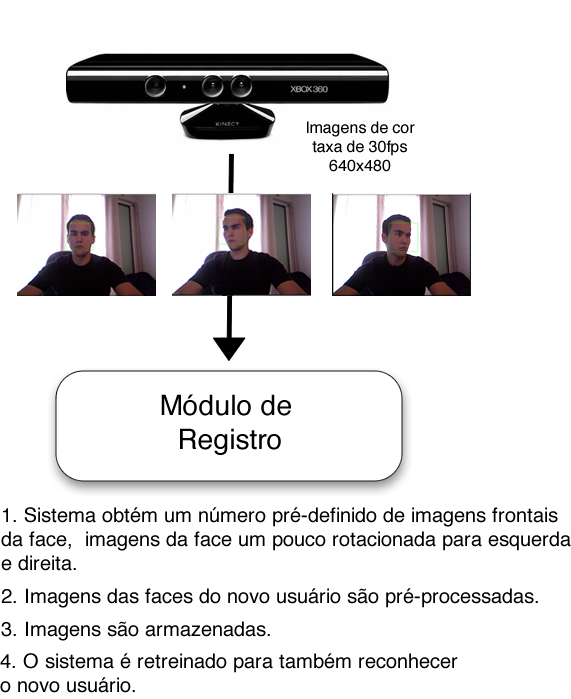
\includegraphics[scale=2.5]{figuras/4.ProblemaEProposta/registro.png}
			\end{center}
			\caption{Etapas de cadastro de um novo usuário no sistema.}
			\label{fig:registro}
		\end{figure}		

		\begin{enumerate}
			\item O novo usuário fica em uma posição fixa e frontal em relação ao \textit{Kinect}. 
			\item O sistema obtém um número pré-definido de imagens frontais do usuário.
			\item O usuário, então, deve rotacionar um pouco a face para a esquerda e o sistema obtém um número pré-definido de imagens do usuário. Depois, deve rotacionar um pouco para direita e o sistema obtém mais imagens do usuário.
			\item As imagens obtidas são processadas: as imagens são convertidas em escala de cinza, novas imagens são criadas recortando a região da face encontrada, as imagens, então, são redimensionadas e equalizadas criando assim uma padrão de tamanho, brilho e contraste nas imagens.
			\item Armazena-se as imagens.
			\item O sistema é treinado para, também, reconhecer esse usuário.
		\end{enumerate}

	Após o treinamento, o sistema \textit{True} reiniciará para que o reconhecimento seja feito utilizando as novas informações obtidas com o treinamento.




	\section{\textit{SmartSpace} Laico}

		O ambiente para o qual o Sistema TRUE será projetado, desenvolvido e testado
		chama-se LAICO (\textbf{LA}boratório de sistemas \textbf{I}ntegrados e
		\textbf{CO}ncorrente), um laboratório do Departamento de Ciência da Computação
		da Universidade de Brasília. O LAICO possui dimensões de, aproximadamente, 
		$\displaystyle 7,67m$ x $\displaystyle 6,45m$ ilustrado pela
		Figura~\ref{fig:laico}.
	
		\begin{figure}[hbt]
			\begin{center}
				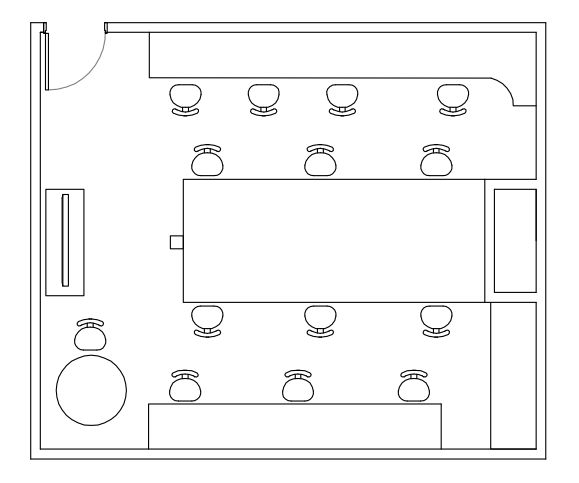
\includegraphics[scale=0.6]{figuras/4.ProblemaEProposta/laico.png}
			\end{center}
			\caption{Planta do \textit{SmartSpace} Laico.}
			\label{fig:laico}
		\end{figure}	


\section{Módulo \textit{UbiquitOS}}















% \chapter{Sistema \textit{TRUE}}
\chapter{Resultados e Análises}
\label{cap:testes}

% - OK Achei o texto introdutório um pouco fraco em apresentar o objetivo do capítulo. 
% 	OK	Acho que vocês poderia focar primeiro que os testes foram para identificar a acurácia do sistema perante seus requisitos (Identificação e Localização). 
% OK		Apresentar o LAICO apenas como o local onde ocorreram os testes. 
% 		Apresentar cada ponto como uma medida/indicador do sistema desenvolvido. 
% 		OK No texto dos 4 testes foque nos objetivos e não no como. Tipo:
% 			Rastreamento: Testar a acurácia do rastreamento e identificação de objetos em situações do cotidiano.
% 			Reconhecimento: Testar a acurácia de identificação dos usuários perante a base de dados.

	Com intuito de identificar a acurácia e as limitações do Sistema TRUE perante seus requisitos (identificação, rastreamento e localização) foram feitos uma série de testes funcionais. Grande parte dos testes foram realizados no LAICO (\textbf{LA}boratório de Sistemas \textbf{I}ntegrados e \textbf{CO}ncorrente), um laboratório do Departamento de Ciência da Computação da Universidade de Brasília. 

	% O LAICO possui dimensões de $\displaystyle 7,67m$ x $\displaystyle 6,45m$ ilustrado pela Figura~\ref{fig:laico}.

	% \begin{figure}[htb]
	% 		\begin{center}
	% 			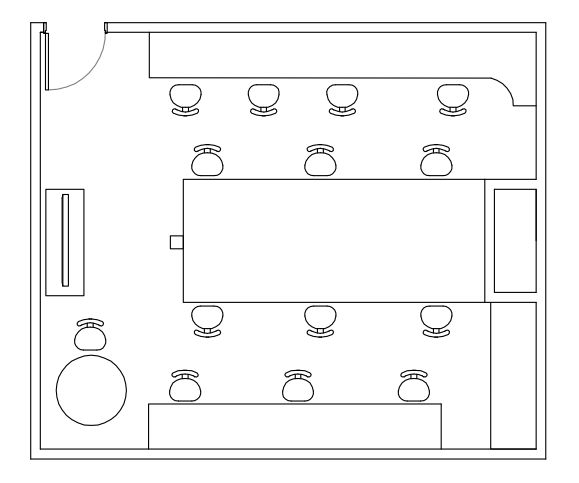
\includegraphics[scale=0.6]{figuras/4.ProblemaEProposta/laico.png}
	% 		\end{center}
	% 		\caption{Planta do \textit{SmartSpace} Laico.}
	% 		\label{fig:laico}
	% 	\end{figure}	

	Cada teste tinha como foco um das funcionalidades do Sistema TRUE:

	\begin{itemize}
		\item \textbf{Rastreamento}: testes funcionais realizados para avaliar a eficiência da detecção de novos usuários e que simulam diferentes situações diárias mostrando como o sistema se comporta quando ocorre oclusões parciais e totais de usuários e quando os mesmos interagem entre si ou com objetos no ambiente.

		\item \textbf{Reconhecimento}: testes realizados para avaliar a acurácia na identificação do usuários perante uma base de dados.

		% diferentes pessoas foram cadastradas no sistema e reconhecidas pelo mesmo. As diferentes identidades obtidas em cada reconhecimento foram inseridas em uma matriz de confusão para avaliar a acurácia do reconhecimento.

		\item \textbf{Localização}: testes realizados para avaliar a precisão do sistema ao estimar a posição dos usuários no ambiente.
	% um objeto foi colocado no ambiente em diferentes posições pre-determinadas e as coordenadas obtidas pelo sistema foram inseridas em gráficos e foram comparadas com as coordeanadas reais avaliando a precisão do sistema.

		\item \textbf{Integração com o middleware \textit{UbiquitOS}}: uma aplicação foi desenvolvida para testar a integração do Sistema TRUE com o middleware \textit{UbiquitOS}, testando os serviços disponíveis e os eventos gerados.

		% uma aplicação foi desenvolvida para o middleware \textit{UbiquitOS}. Ela consome alguns serviços e eventos produzidos pelo driver \textit{UserDriver} que são comparados com as informações reais.
	\end{itemize}

\section{Rastreamento dos Usuários}

	O rastreamento é fundamental para o funcionamento correto do sistema uma vez que é responsável por rastrear os usuários no ambiente, determinar a sua localização física em relação ao sensor \textit{Kinect} e gerenciar suas identidades. Portanto, foi realizado uma série de testes funcionais para determinar suas limitações.

	Os primeiros testes realizados foram para testar a eficiência da detecção de novos usuários no ambiente. Os testes foram feitos simulando a entrada de um usuário na cena por diferentes ângulos e analisando o momento em que o mesmo era detectado. Em todos os testes o usuário era detectado antes mesmo de entrar na área de visão do sistema por completo, como mostrado na Figura~\ref{fig:testes_deteccao}.
	
		\begin{figure}[htb]
			\begin{center}
				\subfloat[] {
					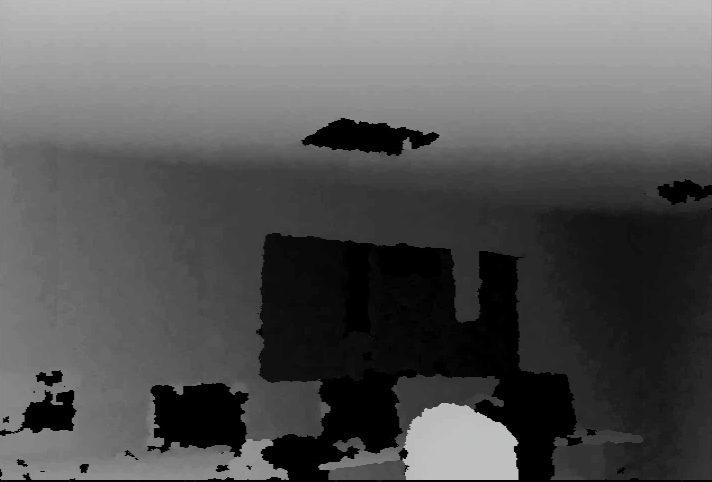
\includegraphics[width=0.25\textwidth]{figuras/5.Testes/deteccao/1.png}}
				\subfloat[] {
					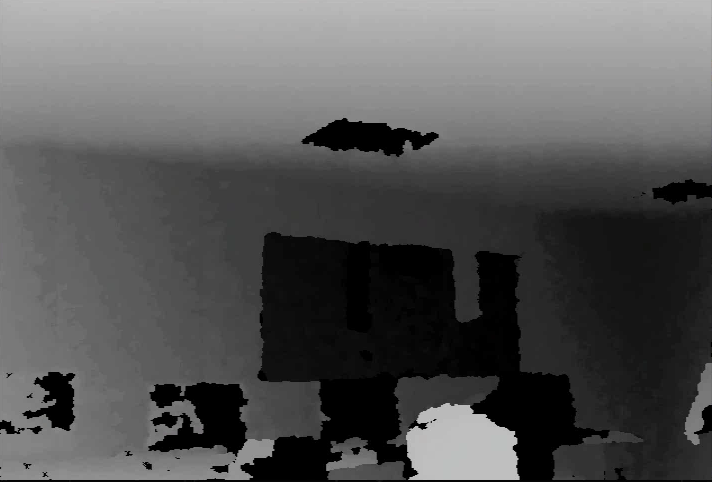
\includegraphics[width=0.25\textwidth]{figuras/5.Testes/deteccao/2.png}}
				\subfloat[] {
					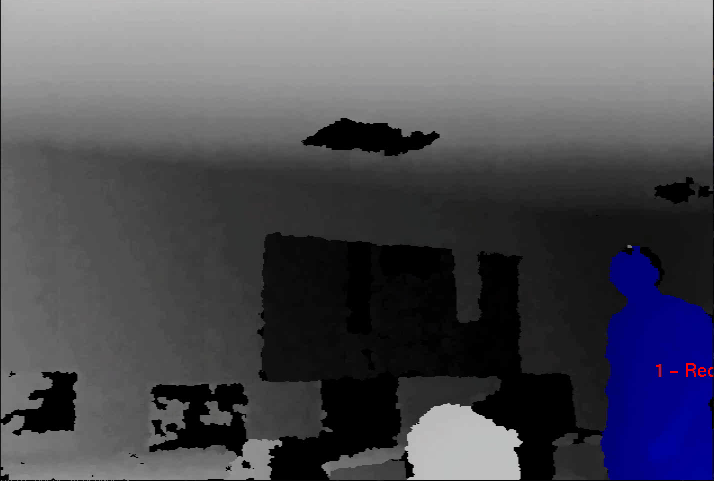
\includegraphics[width=0.25\textwidth]{figuras/5.Testes/deteccao/3.png}}
				\subfloat[] {
					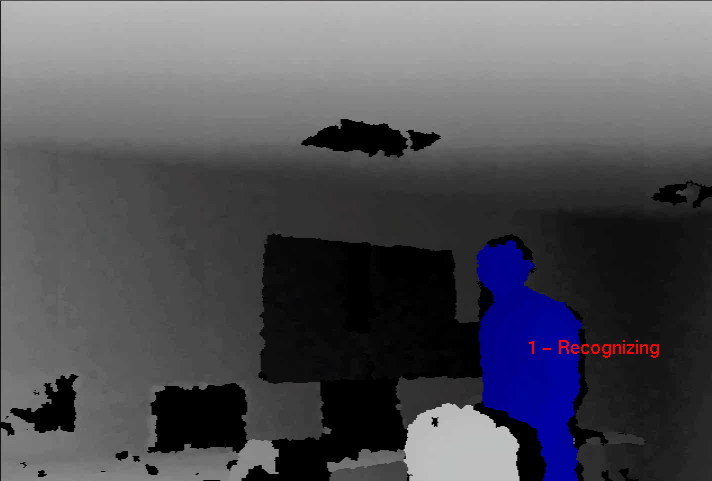
\includegraphics[width=0.25\textwidth]{figuras/5.Testes/deteccao/4.png}}
			\end{center}
			\caption{Momento em que um novo usuário foi detectado pelo Sistema TRUE.}
			\label{fig:testes_deteccao}
		\end{figure}

	Também foram realizados testes para tentar avaliar o impacto da oclusão no rastreamento. Em alguns testes um usuário se posicionava no ambiente com intuito de ocultar totalmente outro usuário rastreado. Com isso, caso o usuário continuasse oculto, o sistema o dava como perdido. Porém, o sistema se mostrou robusto em casos que a oclusão era parcial, como mostrado na Figura~\ref{fig:testes_oclusao_sucesso} Em outros testes, foi simulada uma situação mais comum: quando um usuário, em movimento, ocultava ou era oculto, por um momento, por outro usuário. Neste caso, o sistema logo conseguia se recuperar e voltar a rastrear o usuário perdido, como mostrado na Figura~\ref{fig:testes_oclusao}. A oclusão era um problema esperado pois o Sistema TRUE utiliza somente um sensor \textit{Kinect} como dispositivo de entrada.
		
		\begin{figure}[htb]
			\begin{center}
				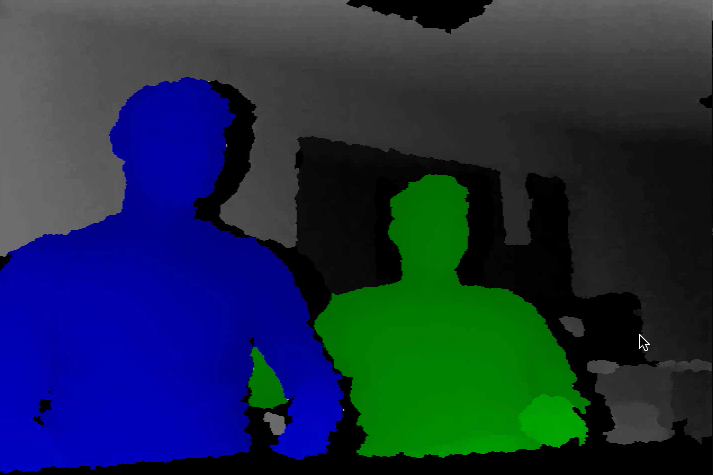
\includegraphics[width=0.75\textwidth]{figuras/5.Testes/oclusao/oclusao_corretamente.png}
			\end{center}
			\caption{Oclusão parcial de dois usuários.}
			\label{fig:testes_oclusao_sucesso}
		\end{figure}
	
		\begin{figure}[htb]
		\begin{center}
				\subfloat[] {
					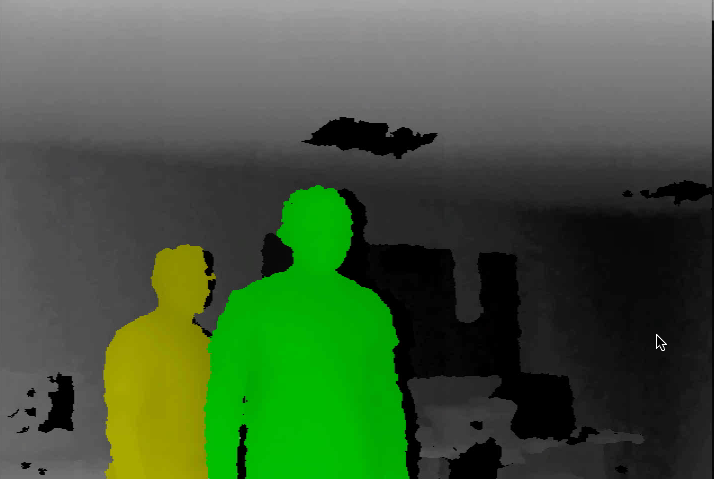
\includegraphics[width=0.19\textwidth]{figuras/5.Testes/oclusao/1.png}}
				\subfloat[] {
					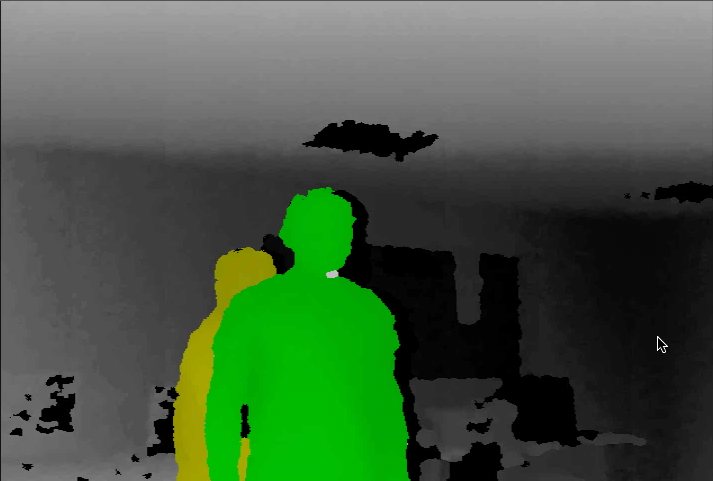
\includegraphics[width=0.19\textwidth]{figuras/5.Testes/oclusao/2.png}}
				\subfloat[] {
					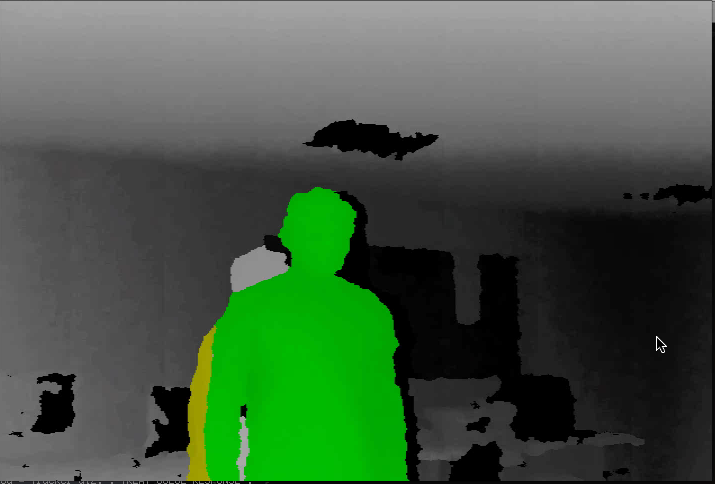
\includegraphics[width=0.19\textwidth]{figuras/5.Testes/oclusao/3.png}}
				\subfloat[] {
					\label{fig:testes_oclusao_ocluso}
					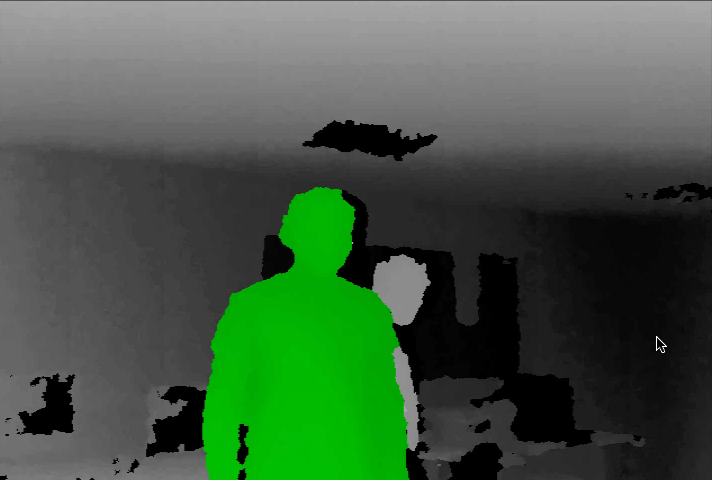
\includegraphics[width=0.19\textwidth]{figuras/5.Testes/oclusao/4.png}}
				\subfloat[] {
					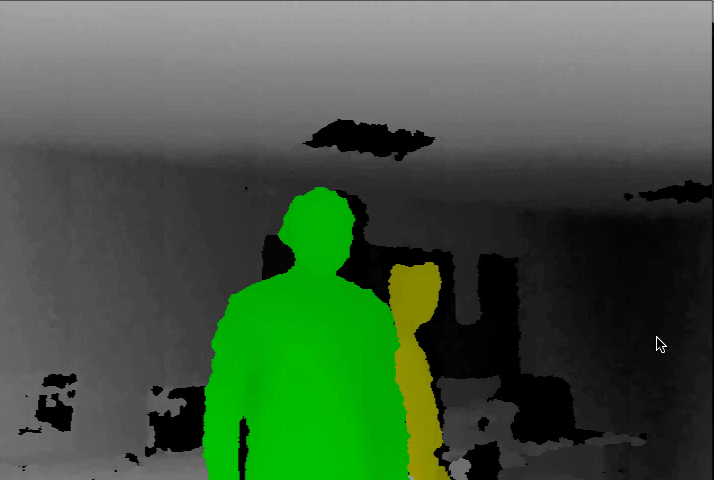
\includegraphics[width=0.19\textwidth]{figuras/5.Testes/oclusao/5.png}}
			\end{center}
			\caption{Oclusão de usuários.}
			\label{fig:testes_oclusao}
		\end{figure}

	Outra caracterísitca importante que foi testada é a abrangência do campo de
	visão do Sistema TRUE. Como já mensionado o sistema utiliza o sensor
	\textit{Kinect} que possui um campo de visão horizontal de 57º. Então, a uma
	distância de, aproximadamente, 4 metros do sensor, o número máximo de usuários
	que cabem no campo de visão sem que haja oclusão são 5 pessoas, como mostrado
	na Figura~\ref{fig:max-pessoas}.

	\begin{figure}[htb]
			\begin{center}
				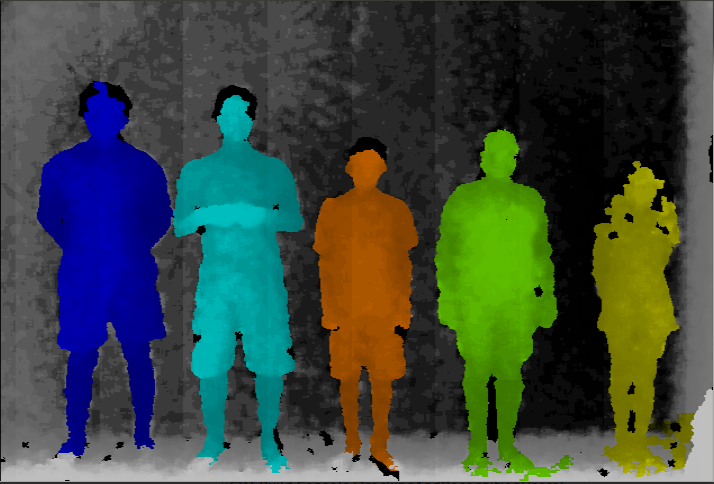
\includegraphics[width=0.4\textwidth]{figuras/5.Testes/oclusao/max-pessoas.png}
			\end{center}
			\caption{Usuários posicionados lado a lado do sensor \textit{Kinect} a uma distância de 4 metros.}
			\label{fig:max-pessoas}
		\end{figure}
		
	Durante os testes realizados com rastreamento foi observado alguns problemas que ocorriam quando o usuário rastreado interagia com objetos ou com outros usuários. Na grande parte das vezes que o usuário interagia com objetos, o Sistema TRUE considerava o objeto como sendo parte do usuário como exemplificado na Figura~\ref{fig:testes_relacionamento_com_objetos}, o que não prejudicou a eficiência do sistema. Já os problemas com interação entre usuários eram bem mais raros, porém o impacto era maior. Esses problemas consistem em algumas ``interferências'' que podiam acontecer quando havia contato entre dois ou mais usuários. A Figura~\ref{fig:testes_relacionamento_com_usuarios} exemplifica melhor essas ``interferências''.
	
		\begin{figure}[htb]
			\begin{center}
				\subfloat[] {
					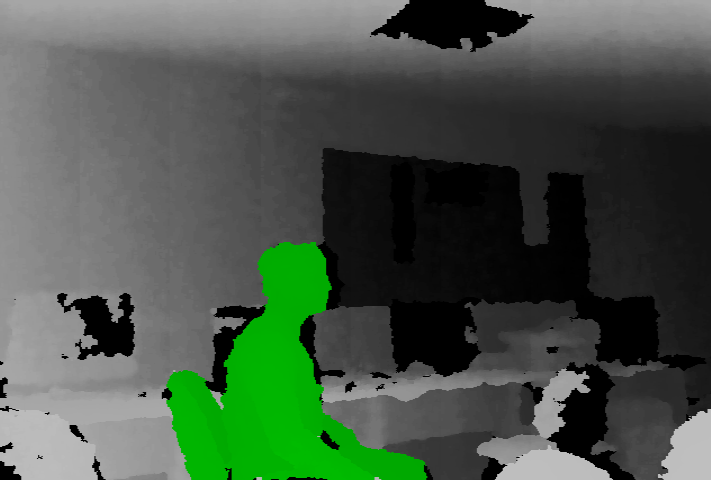
\includegraphics[width=0.37\textwidth]{figuras/5.Testes/relacionamento_com_objetos/1.png}}
				\subfloat[] {
					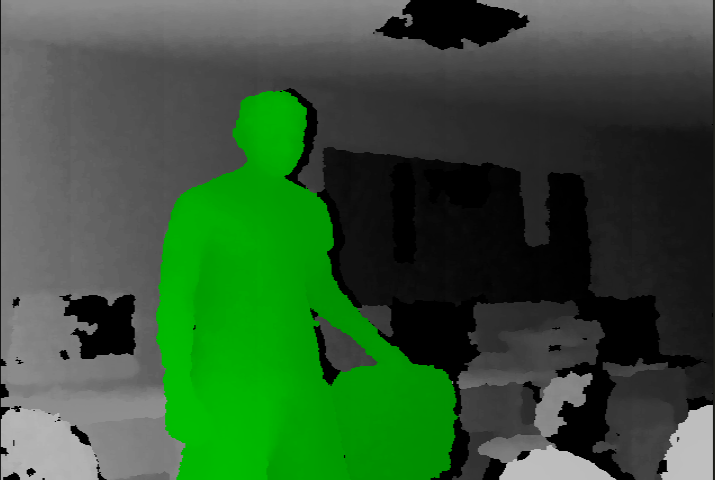
\includegraphics[width=0.37\textwidth]{figuras/5.Testes/relacionamento_com_objetos/2.png}}
			\end{center}
			\caption{Usuários sendo rastreado conjuntamente com os objetos que
			interagem.}
			\label{fig:testes_relacionamento_com_objetos}
		\end{figure}
		
		\begin{figure}[htb]
			\begin{center}
				\subfloat[] {
					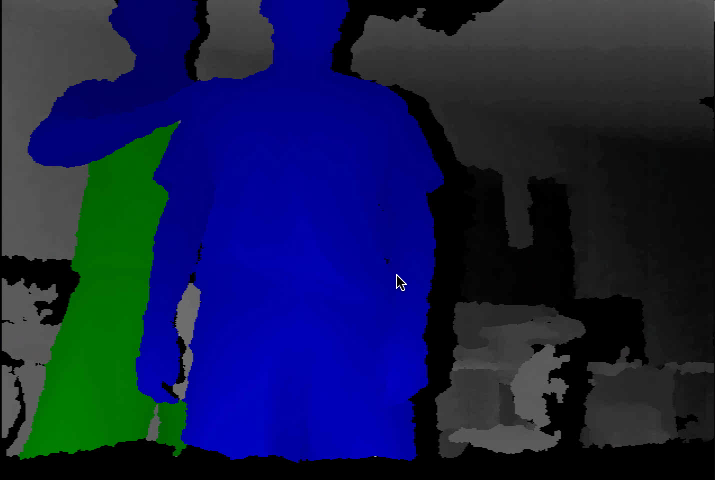
\includegraphics[width=0.32\textwidth]{figuras/5.Testes/relacionamento_com_pessoas/1.png}}
				\subfloat[] {
					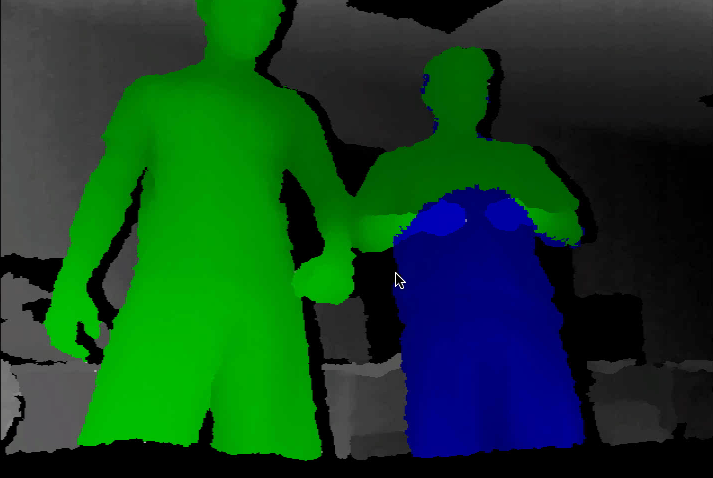
\includegraphics[width=0.32\textwidth]{figuras/5.Testes/relacionamento_com_pessoas/2.png}}
				\subfloat[] {
					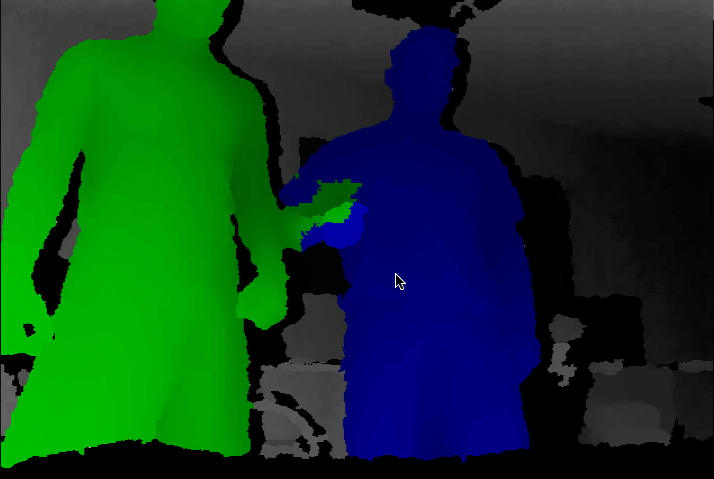
\includegraphics[width=0.32\textwidth]{figuras/5.Testes/relacionamento_com_pessoas/3.png}}
			\end{center}
			\caption{Usuários sofrendo interferência dos que estão ao seu redor.}
			\label{fig:testes_relacionamento_com_usuarios}
		\end{figure}

	Apesar dos problemas relatados, o rastreamento conseguiu, na maioria dos testes, atender as necessidades rastreando os diversos usuários no ambiente em suas atividades diárias, como mostrado na Figura~\ref{fig:varios-usuarios-ambiente}.

		\begin{figure}[htb]
			\begin{center}
				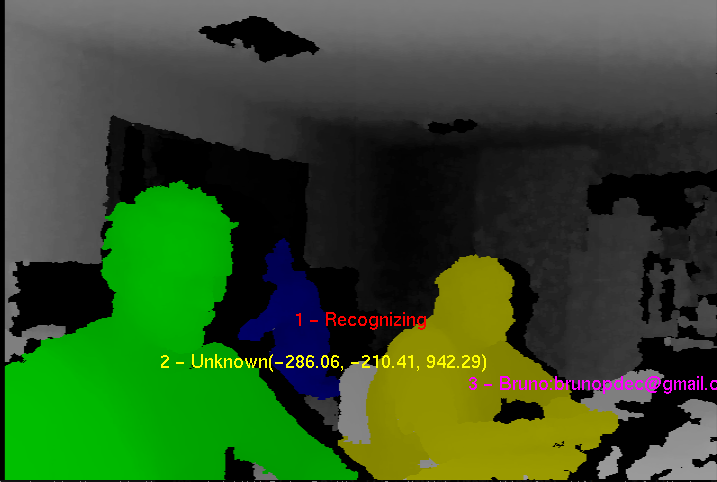
\includegraphics[scale=0.5]{figuras/5.Testes/oclusao/usuarios-rastreados.png}
			\end{center}
			\caption{Usuários rastreados pelo Sistema TRUE.}
			\label{fig:varios-usuarios-ambiente}
		\end{figure}
		
	

\section{Localização dos Usuários}

O Sistema TRUE obtém a localização dos usuários no ambiente por meio de coordenadas dos mesmos em relação ao \textit{Kinect}. Para saber o quanto essas coordenadas são confiáveis foram realizados alguns testes que resultaram em gráficos que comparam as coordenadas obtidas pelo sistema e as coordenadas reais.

As coordenadas $\displaystyle (x, y, z)$ obtidas pelo sistema são coordenas de um plano cartesiano de três dimensões em que o ponto $\displaystyle (0, 0, 0)$ corresponde a posição do \textit{Kinect}. Os valores das coordenadas que realmente são utilizadas para estimar a localização do usuário no ambiente são os valores nos eixos $\displaystyle x$ e $\displaystyle z$. Os valores do eixo $\displaystyle y$ correspondem somente a altura do centro de massa geométrico do usuário rastreado. Portanto, os testes desenvolvidos aferiram somente os valores obtidos pelo Sistema TRUE nos eixos $\displaystyle x$ e $\displaystyle z$.

\subsection{Teste dos valores no eixo $\displaystyle z$}

	Os valores obtidos no eixo $\displaystyle z$ correspondem aos valores de profundidade do usuário rastreado em relação ao \textit{Kinect}. Portanto, para testar a precisão do Sistema TRUE foi realizado o seguinte teste: um objeto (uma caixa de papelão) foi colocada em frente ao sensor, como mostrado na Figura~\ref{fig:teste-z}, em diferentes distâncias do mesmo (1 metro, 2 metros, 3 metros, 4 metros, 4,057 metros). Para cada distância, foram anotados alguns valores obtidos pelo sistema, mostrados na Tabela~\ref{tab:valores-z}, e foram obtidas diferentes imagens do Sistema TRUE mostradas na Figura~\ref{fig:distancias}. Então esses valores foram inseridos em um gráfico e comparado com os valores reais.

	\begin{figure}[htb]
		\begin{center}
			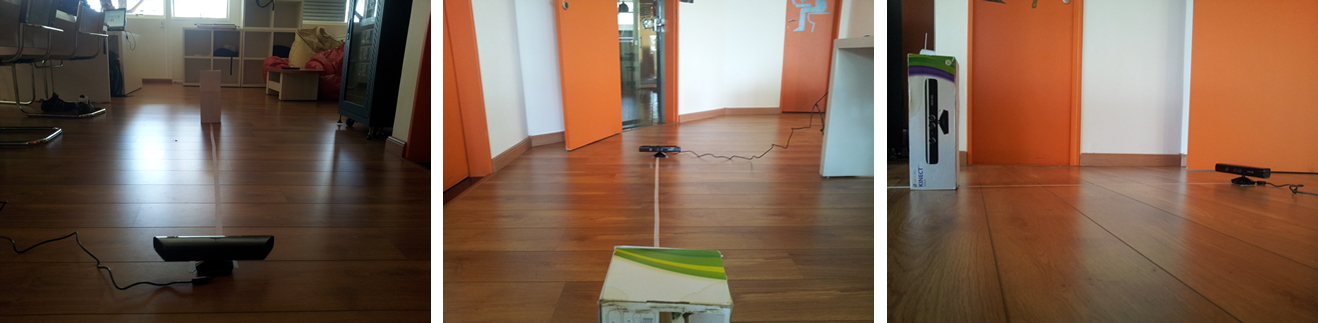
\includegraphics[scale=0.35]{figuras/5.Testes/teste-eixoz.png}
		\end{center}
		\caption{Fotos retiradas no teste realizado para aferir os valores obtidos no eixo $\displaystyle z$.}
		\label{fig:teste-z}
	\end{figure}

	\begin{figure}[htb]
		\begin{center}
			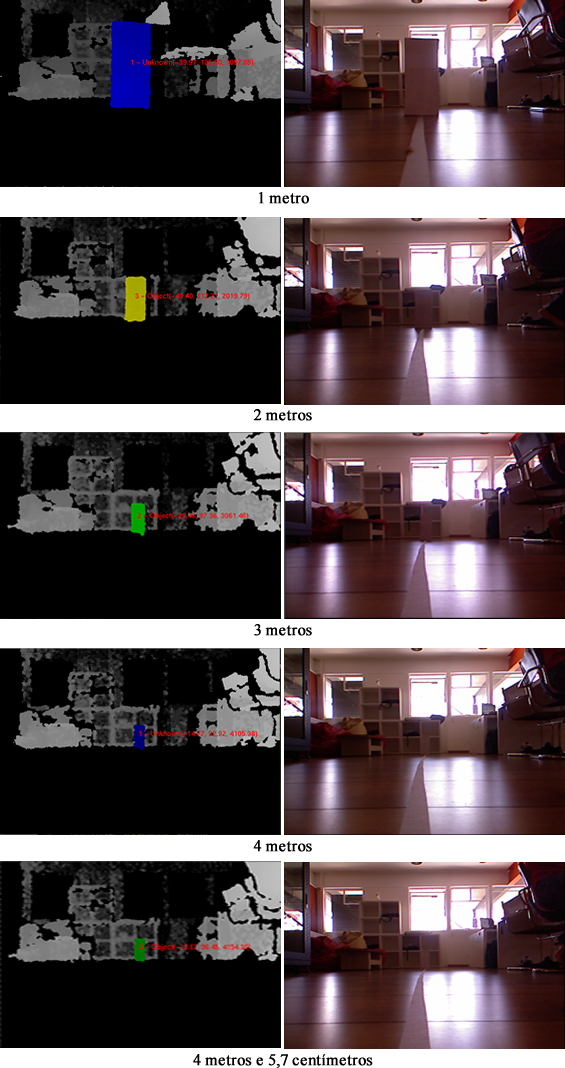
\includegraphics[scale=0.6]{figuras/5.Testes/eixoz-imgs.png}
		\end{center}
		\caption{Fotos retiradas no teste realizado para aferir os valores obtidos no eixo $\displaystyle z$.}
		\label{fig:distancias}
	\end{figure}

		\begin{table}[h]
		\begin{center}
			\caption{Valores obtidos pelo Sistema TRUE.}
			\begin{tabular}{|c|c|c|c|c|}
				\hline \bf Distância do objeto ao \textit{Kinect} (mm) & \multicolumn{4}{|c|}{\bf Valores obtido pelo Sistema TRUE (mm)} \\
				\hline
				\hline 1000,00 & 1007,56 & 1006,64 & 1003,21 & 1007,56 \\
				\hline 2000,00 & 2020,27 & 2021,17 & 2020,55 & 2020,48 \\
				\hline 3000,00 & 3058,70 & 3057,60 & 3062,01 & 3059,10 \\
				\hline 4000,00 & 4115,31 & 4110,25 & 4111,59 & 4114,80 \\
				\hline 4057,00 & 4166,35 & 4163,83 & 4166,45 & 4168,75 \\
				\hline
			\end{tabular}
		\end{center}
		\label{tab:valores-z}
	\end{table}

	Os valores obtidos no teste foram inseridos em um gráfico representado pela Figura~\ref{fig:grafico-z}. Neste gráfico existem duas retas: uma reta preta que representa valores ideias que batem com os valores reais; e uma reta vermelha que representa os valores obtidos pelo sistema. Como observado, a medida que o objeto se afasta do \textit{Kinect} as diferenças entre os valores reais e os valores obtidos aumetam. Contudo, essa diferença é de poucos centímetros.

	\begin{figure}[htb]
		\begin{center}
			\includegraphics[scale=0.4]{figuras/5.Testes/grafico-eixo-z.png}
		\end{center}
		\caption{Gráfico comparativo entre os valores obtidos pelo Sistema TRUE e os valores reais.}
		\label{fig:grafico-z}
	\end{figure}

	Pelos resultados deste teste, pode-se concluir que o Sistema TRUE fornece informações sobre localização dos usuários bem precisas e confiáveis podendo ter erros de poucos centímetros que não prejudicam a integridade das informações. 

	Através deste teste, também foi possível obter a distância máxima e mínima que o usuário deve estar do \textit{Kinect} para que o sistema consiga rastrear-lo e estimar sua localização. A distância mínima é de $\displaystyle 48,3 cm$ e a máxima de $\displaystyle 4,057 m$.

\subsection{Teste dos valores no eixo $\displaystyle x$}



















\section{Identificação dos Usuários}
	
	Os usuários são identificados através do metodo conhecido como
	Eigenfaces~\ref{sec:reconhecimento}. Os usuários são identificados por suas
	labels de cadastro e a cada reconhecimento é associado a essa label uma
	confiança. Para validar a confiabilidade da identificação será usado a matriz
	de confusão para representar os dados dos testes.
	
	\begin{table}[H]
		\begin{center}
			\caption{Matriz de confusão para apresentar os resultados obtidos.}
			\begin{tabular}{|c|c|c|c|c|c|c|c|c|c|}
				\hline \bf X & \bf Tales & \bf Danilo & \bf Fabrício & \bf Ricardo & \bf
				Bruno & \bf Estevão & \bf Guto & \bf Tainá & \bf Tanyssa \\
				\hline \bf Tales & & & & & & & & & \\
				\hline \bf Danilo & & & & & & & & & \\
				\hline \bf Fabrício & & & & & & & & & \\
				\hline \bf Ricardo & & & & & & & & & \\
				\hline \bf Bruno & & & & & & & & & \\
				\hline \bf Estevão & & & & & & & & & \\
				\hline \bf Guto & & & & & & & & & \\
				\hline \bf Tainá & & & & & & & & & \\
				\hline \bf Tanyssa & & & & & & & & & \\
				\hline
			\end{tabular}
		\end{center}
		\label{tab:tabelaRequisitosTeoricos}
	\end{table}


\section{Integração com Middleware \textit{uOS}}

	A integração do Middleware \textit{uOS} com o Sistema TRUE consiste em um \textit{driver} desenvolvido para que ambos possam se comunicar. Este \textit{driver} foi nomeado de \textit{UserDriver} que foi apresentado na Seção~\ref{sec:modulo-integracao}. Com intuito de exemplificar a utilização do \textit{UserDriver} e testar a integração do Sistema TRUE com o middleware \textit{uOS} foi desenvolvido uma aplicação para o middleware chamada \textit{UserApp}. Esta aplicação registra um \textit{listener} para ``escutar'' os eventos do \textit{UserDriver} chamado \textit{UserListener}. 

	Como aplicação o \textit{UserApp} apenas se inscreve para receber os eventos gerados pelo \textit{UserDriver}. Já o \textit{UserListener}, como \textit{listener}, espera os eventos serem gerados e realiza duas análises: analisa o evento (novo usuário detectado, usuário perdido, ou reconhecimento realizado) e analisa quanto tempo cada usuário está parado no mesmo lugar.

		% \begin{figure}[hbt]
		% 	\begin{center}
		% 		\includegraphics[scale=0.6]{figuras/5.Testes/diagrama-classe-user-ap.png}
		% 	\end{center}
		% 	\caption{Diagrama de Classe da aplicação \textit{UserApp}.}
		% 	\label{fig:diagrama-userapp}
		% \end{figure}

		% \begin{figure}[hbt]
		% 	\begin{center}
		% 		\includegraphics[scale=0.6]{figuras/5.Testes/diagrama-classe-user-listener.png}
		% 	\end{center}
		% 	\caption{Diagrama de Classe do \textit{listener} \textit{UserListener}.}
		% 	\label{fig:diagrama-userlistener}
		% \end{figure}

	% Basicamente, quando o \textit{UserListener} obtém os eventos do \textit{UserDriver}, ele envia mensagens pelo Twitter~\cite{twitter} para os usuários no ambiente, conforme o evento recebido. Para enviar as mensagens pelo Twitter foi utilizado a biblioteca \textit{twitter4j}~\cite{twitter4j}. A Figura~\ref{fig:diagrama-tweet} mostra o fluxo básico de execução do \textit{listener} e as mensagens padrões para cada tipo de evento recebido. 

	Basicamente, quando o \textit{UserListener} é inicializado ele obtém acesso ao twitter e se registra para escutar os eventos gerados pelo \textit{UserDriver}. Para cada evento obtido, ele envia mensagens pelo Twitter~\cite{twitter} para os usuários no ambiente. Para eventos de ``novo usuário detectado'' e ``usuário perdido'', ele envia mensagens de boas vindas e de despedidas respectivamente. Como mencionado na Seção~\ref{sec:modulo-integracao}, o \textit{UserDriver} também gera eventos de atualização dos dados dos usuários. Quando estes eventos são gerados, o \textit{UserListener} verifica se houve atualização na identidade do usuário e se o mesmo está a mais de uma hora no mesmo lugar. Caso esteja, ele envia mensagens aos usuários informando estes acontecimentos. Este fluxo de execução e as estruturas das mensagens enviadas são mostrados na Figura~\ref{fig:diagrama-tweet}. Para enviar as mensagens pelo Twitter foi utilizado a biblioteca \textit{twitter4j}~\cite{twitter4j}.

	\begin{figure}[hbt]
		\begin{center}
			\includegraphics[scale=0.45]{figuras/5.Testes/diagrama-user-tweet.png}
		\end{center}
		\caption{Fluxo básico de execução do \textit{listener} \textit{UserListener}.}
		\label{fig:diagrama-tweet}
	\end{figure}

	Testes funcionais foram feitos com a aplicação mostrando que o \textit{driver} consegue
	obter os dados íntegros do Sistema TRUE e gerar os eventos de maneira praticamente
	instantânea. Algumas vezes as mensagens demoravam a chegar ao Twitter,
	geralmente nos horários de pico quando o Twitter operava próximo ao limite
	da sua capacidade. A Figura~\ref{fig:tweets} mostra as mensagens geradas
	pela aplicação em um teste funcional, onde Danilo, um usuário cadastrado,
	entra no ambiente senta em uma mesa com seu notebook permanecendo no mesmo
	lugar por mais de uma hora, e logo depois deixa o ambiente.

	\begin{figure}[hbt]
			\begin{center}
				\includegraphics[scale=0.6]{figuras/5.Testes/tweets.png}
			\end{center}
			\caption{Exemplo das mensagens enviadas pelo Twitter aos usuários no ambiente.}
			\label{fig:tweets}
		\end{figure}	












\chapter{Conclusões}
\label{cap:conclusao}


% O objeto de estudo eh o uos exolica. tendo em vista que o uos nao possui

% pouco de impl

Dentre as diversas informações de contexto que podem ser obtidas em ambientes
inteligentes, as informações que contém as identidades e as posições dos
usuários são fundamentais para que o ambiente possa tomar decisões em prol dos
usuários de modo a realmente se tornar inteligente. A obtenção dessas
informações já é objeto de pesquisa, porém a maioria das soluções encontradas
foram projetadas para funcionar em ambientes rigidamente definidos. Com isso,
não seria adequado tentar incorporar soluções como estas em um ambiente com
diferentes dimensões, condições de iluminação, posição dos móveis, diferentes
sensores pois este resultaria em um cenário diferente.

O objeto de estudo deste trabalho é o middleware \textit{uOS}. Ele é uma
implementação de um middleware para auxílio de aplicações para ambiente de
computação ubíqua, cuja proposta é compatível com os conceitos apresentados
pela \textit{DSOA} (\textit{Device Service Oriented
Architecture})~\cite{fabriciobuzzeto}. O foco do \textit{uOS} está na
adaptabilidade de serviços em um ambiente de computação ubíqua, de modo que os
serviços dos dispositivos presentes no ambiente possam ser oferecidos e
compartilhados.

Tendo em vista que o middleware \textit{uOS} ainda não obtém informações de identidades e localizações dos usuários no ambiente, este
trabalho propõe a implementação de um sistema de rastreamento, localização e reconhecimento que disponibiliza estas informações ao \textit{uOS}. Este Sistema é chamado de Sistema TRUE (\textit{\textbf{T}racking and \textbf{R}ecognizing \textbf{U}sers in the \textbf{E}nvironment}) que utiliza o sensor \textit{Kinect} como dispositivo de entrada.

O rastreamento é fundamental para o funcionamento correto do Sistema TRUE. Ele é responsável por detectar e rastrear os usuários servindo como base para que novas informações possam ser obtidas. O Sistema TRUE se mostrou eficaz na detecção de novos usuários que são detectados antes mesmo de entrarem por completo no campo de visão e se revelou robusto em casos de oclusões parciais. Contudo, casos de oclusões totais prejudicam a eficácia do sistema. Além disso, o campo de visão se mostrou limitado rastreando no máximo 5 pessoas simultâneamente à uma distância máxima de 4,057 metros.

O Sistema TRUE estimava a posição dos usuários por meio de coordenadas em relação ao sensor \textit{Kinect}. Portanto, fixando a posição do sensor é possível obter a localização física dos usuários no ambiente. As coordenadas obtidas se mostraram bem precisas e confiáveis apresentando erros de poucos centímetros que aumentam juntamente com a distância entre o usuário e o sensor. 

Para identificar os usuários no ambiente, o Sistema TRUE realiza reconhecimento
facial dos usuários através de imagens de cor de suas faces. Os testes
realizados mostraram que a estratégia utilizada no cadastro dos usuários tem
grande impacto nos resultados do reconhecimento. Utilizando-se várias imagens
em diferentes ângulos, com diferentes poses e expressões faciais no cadastro de
cada usuário, obtém-se melhores resultados. Ainda assim, a variação de pose e
ângulo das faces obtidas dos usuários no ambiente prejudicam o reconhecimento
facial implementado no Sistema TRUE.

\section{Trabalhos Futuros}

Era esperado ao término deste trabalho que o sistema rastreasse, identificasse e localizasse os usuários no ambiente inteligente. No entanto, foi mostrado que há limitações referentes ao rastreamento e identificação. Dada a implementação do Sistema TRUE e suas funcionaldiades da forma que foi definida, os próximos passos seriam:

\begin{itemize}
	\item ampliação do número de sensores \textit{Kinect} utilizados pelo sistema para que se torne mais robusto aos problemas causados pela oclusão e pelo campo de visão limitado.
	\item utilização de técnicas que torne o reconhecimento facial mais robusto em relação as constantes variações de poses e ângulos das faces capturadas.
\end{itemize}






\postextual

\bibliographystyle{plain}

\bibliography{bibliografia}

\appendix
\chapter{Kinect}
\label{sec:kinect}

% O Kinect, mostrado na Figura \ref{kinect}, é o nome de um projeto da Microsoft para seu console de videogame Xbox 360, que tem ainda como colaboradora a empresa Prime Sense. O projeto visa criar uma nova tecnologia capaz de permitir aos jogadores interagir com os jogos eletrônicos sem a necessidade de ter em mãos um controle(\textit{joystick}), inovando no campo da jogabilidade.

O \textit{Kinect}, mostrado na Figura~\ref{kinect}, é o nome do acessório desenvolvido pela Microsoft com a colaboração da Prime Sense para seu console de videogame Xbox 360. Tal acessório permite aos jogadores interagir com os jogos eletrônicos sem a necessidade de interagir diretamente com um controle (\textit{joystick}). Devido a este fato o \textit{Kinect} foi considerado uma grande inovação no campo da jogabilidade.

	\begin{figure}[hbt]
		\begin{center}
		\includegraphics[scale=0.07]{figuras/Apendice/kinect.JPG}
		\end{center}
		\caption{Sensor Kinect da Microsoft.}
		\label{kinect}
	\end{figure}

	A Microsoft define o \textit{Kinect} como ``jogos sem necessidade de controle e experiência de entretenimento''. Porém, seu uso e inovação não se limita apenas no campo dos jogos eletrônicos (15).

	O \textit{Kinect} possui as seguintes especificações técnicas:

	\begin{itemize}
		\item Sensor
			\begin{itemize}
				\item Lentes com detecção de cores e profundidade
				\item Microfone de voz
				\item Motor de inclinação para ajuste do sensor
			\end{itemize}
		\item Campo de visão
			\begin{itemize}
				\item Campo de visão horizontal: 57 graus
				\item Campo de visão vertical: 43 graus
				\item Alcance físico da inclinação: (+/-) 27 graus
				\item Um alcance máximo de aproximadamente $\displaystyle 4.5$ metros para câmera de profundidade. 
			\end{itemize}
		\item Fluxo de Dados
			\begin{itemize}
				\item 320x240 16-bit depth a 30FPS
				\item 640x480 32-bit color a 30FPS
				\item 16-bit áudio a 16 kHz
			\end{itemize}
	\end{itemize}

Seu hardware é composto por câmeras que obtém imagens de cor, som e que utiliza iluminação infravermelha (IR) para obter dados de profundidade~\cite{kinect}. A Figura \ref{kinect_interno} apresenta a organização interna do \textit{Kinect} em alto nível.

	\begin{figure}[hbt]
		\begin{center}
			\includegraphics[scale=0.8]{figuras/2.FundamentacaoTeorica/kinect_interno.png}
		\end{center}
		\caption{Organização interna do Kinect~\cite{kinect}.}
		\label{kinect_interno}
	\end{figure}

Um chip especializado é responsável pelo processamento dos dados fornecidos pela câmera de profundidade correlacionando-os com as imagens de cor. O software interno ao \textit{Kinect} combina cada pixel com sua profundidade, processa os dados e os envia a máquina por meio de uma interface USB na forma de mapas de profundidades e imagens de cor~\cite{kinect}.


\chapter{Processamento da imagem}
\label{apend:processamento}

As etapas de processamento da imagem utilizadas nesse trabalho consistem na conversão em escala de cinza, corte, redimensionamento e equalização da mesma. Neste apêndice são mostrado trechos de códigos que implementam tais etapas utilizando a biblioteca \textit{OpenCV}.

\section{Escala de Cinza}

		\begin{lstlisting}[caption=Conversão de uma imagem para escala de cinza., label=list:grey-scale]
		IplImage* imageToGreyscale(const IplImage *imageSrc) {
			IplImage *imageGrey;

			// cria uma nova imagem do mesmo tamanho que a imagem passada como parametro e de 1 canal.
			imageGrey = cvCreateImage(cvGetSize(imageSrc), IPL_DEPTH_8U, 1);

			//converte o espaco de cor de imageSrc para o espaco de cor (cinza) da imageGrey
			cvCvtColor(imageSrc, imageGrey, CV_BGR2GRAY);

			return imageGrey;
		}
		\end{lstlisting}

\section{Corte da Imagem}

	\begin{lstlisting}[caption=Corte de uma imagem., label=list:crop]
		IplImage* crop(const IplImage *img, const CvRect region) {
			IplImage *imageTmp;
			IplImage *imageRGB;
			CvSize size;
			size.height = img->height;
			size.width = img->width;

			if (img->depth != IPL_DEPTH_8U) {
				printf("ERROR: img->depth de %d desconhecido ao inves de 8 bits por pixel passado a crop().\n", img->depth);
				exit(1);
			}

			// cria uma nova imagem (colorida ou em cinza) e copia os conteudos da imagem nela.
			imageTmp = cvCreateImage(size, IPL_DEPTH_8U, img->nChannels);
			cvCopy(img, imageTmp, NULL);

			// cria uma nova imagem da regiao detectada
			// seta a região de interesse que é ao redor da face
			cvSetImageROI(imageTmp, region);

			//copia a imagem de interesse na nova iplImage (imageRGB) e a retorna
			size.width = region.width;
			size.height = region.height;
			imageRGB = cvCreateImage(size, IPL_DEPTH_8U, img->nChannels);
			cvCopy(imageTmp, imageRGB, NULL);//copia somente a regiao

			cvReleaseImage(&imageTmp);
			return imageRGB;
		}
	\end{lstlisting}

\section{Redimensionamento}

	\begin{lstlisting}[caption=Redimensionamento de uma imagem., label=list:resize]
		IplImage* resize(const IplImage *origImg, int newWidth, int newHeight) {
			IplImage *outImg = 0;
			int origWidth, origHeight;

			if (origImg) {
				origWidth = origImg->width;
				origHeight = origImg->height;
			}

			if (newWidth <= 0 || newHeight <= 0 || origImg == 0 || origWidth <= 0 || origHeight <= 0) {
				printf("ERROR: Tamanho %dx%d desejado para imagem invalido\n.", newWidth, newHeight);
				exit(1);
			}

			// modifica as dimensoes da imagem, mesmo se a proporcao mude
			outImg = cvCreateImage(cvSize(newWidth, newHeight), origImg->depth, origImg->nChannels);
			cvResetImageROI((IplImage*) origImg);
			if (newWidth > origImg->width && newHeight > origImg->height) { // aumentar a imagem
				//CV_INTER_LINEAR muito boa para aumentar a imagem
				cvResize(origImg, outImg, CV_INTER_LINEAR); 

			} else { //diminuir a imagem
				//CV_INTER_AREA muito boa para diminuir a imagem, porem pessima para aumenta-la
				cvResize(origImg, outImg, CV_INTER_AREA);
			}

			return outImg;
		}
	\end{lstlisting}

\section{Equalização}

	\begin{lstlisting}[caption=Equalização de uma imagem., label=list:equalizacao]
		//cria uma imagem limpa na escala de cinza
		equalizedImg = cvCreateImage(cvGetSize(sizedImg), 8, 1); 

		// metodo que realiza "equalização de histograma"
		// normalizando o brilho e aumentando o contraste
		cvEqualizeHist(sizedImg, equalizedImg);
	\end{lstlisting}	

	% TODO : remover os acentos dentro dos lstlisting
\chapter{JNI}
\label{apend:jni}

JNI (\textit{Java Native Interface}) é uma \textit{framework} que permite que
aplicações em Java possam chamar e serem chamadas por aplicações nativas e
bibliotecas escritas em outras linguagem tal como C, C++ e Assembly.
O propósito desta ferramenta é oferecer a possibilidade de que programadores
possam implementar funcionalidades não disponibilizadas pela API padrão do Java
ou até mesmo melhorar as já implementadas seja por questão de desempenho,
segurança ou outros.

A implementação de métodos nativos exige a criação de uma função seguindo a estrutura
\ref{list:estruturaJNI}. Quando a JVM executar o método ela invocará a função
definida e passará os parâmetros conforme o esperado \cite{jniDoc}. 

	\begin{lstlisting}[caption=HelloWorld.java., label=list:estruturaJNI]	
		JNIEXPORT void JNICALL Java_ClassName_MethodName(JNIEnv *env, jobject obj) {
			/*Implement Native Method Here*/
		}
	\end{lstlisting}
	
\section{HelloWorld}

	Os arquivos \ref{list:helloWorldJava}, \ref{list:helloWorldH},
	\ref{list:helloWorldC} e \ref{list:make} exemplificam os fontes envolvidos na criação de uma aplicação utilizando JNI. De posse destes arquivos a execução do comando a seguir finaliza o processo \cite{jniDoc}.

	% Para criar o primeiro programa utilizando a JNI basta criar os arquivos
	% \ref{list:helloWorldJava}, \ref{list:helloWorldH},
	% \ref{list:helloWorldC} e \ref{list:make} e no console executar \cite{jniDoc}:
	
	\textit{chmod +x make.sh}
	
	\textit{./make.sh}


	\begin{lstlisting}[caption=HelloWorld.java., label=list:helloWorldJava]
	class HelloWorld {
			static {
				System.loadLibrary("HelloWorld");
	    }
	    
	    private native void print();
	        
	    public static void main(String[] args) {
	    	new HelloWorld().print();
	    }   
	}
	\end{lstlisting}
	
	\begin{lstlisting}[caption=HelloWorld.h., label=list:helloWorldH]
	
		/* DO NOT EDIT THIS FILE - it is machine generated */
		#include <jni.h>
		/* Header for class HelloWorld */
		 
		#ifndef _Included_HelloWorld
		#define _Included_HelloWorld
		#ifdef __cplusplus
		extern "C" {
		#endif
		/*
		 * Class:     HelloWorld
		 * Method:    print
		 * Signature: ()V
		 */
		JNIEXPORT void JNICALL Java_HelloWorld_print(JNIEnv *, jobject);
		 
		#ifdef __cplusplus
		}
		#endif
		#endif
	\end{lstlisting}
		
	\begin{lstlisting}[caption=HelloWorld.c., label=list:helloWorldC]
		#include "jni.h"
		#include <stdio.h>
		#include "HelloWorld.h"
		 
		JNIEXPORT void JNICALL Java_HelloWorld_print(JNIEnv *env, jobject obj) {
		    printf("Hello World!\n");
		    return;
		}
	\end{lstlisting}
	
	\begin{lstlisting}[caption=make.sh., label=list:make]
		#!/bin/sh
		export LD_LIBRARY_PATH=$LD_LIBRARY_PATH:.
		javah HelloWorld
		gcc -shared -Wl,-soname,HelloWorld -o libHelloWorld.so HelloWorld.c \
			-I/usr/lib/jvm/java-6-openjdk/include \
			-I/usr/lib/jvm/java-6-openjdk/include/linux
		javac HelloWorld.java
		java HelloWorld
	\end{lstlisting}



\end{document}


